\setcounter{chapter}{2}

\chapter{{Application de la méthodologie AMIS au cas expérimental FFT07}}

Dans ce chapitre, nous appliquons l'algorithme AMIS à un problème STE avec des données d'observations réelles issues d'une campagne expérimentale de mesures. Nous présentons dans un premier temps le contexte de la campagne, puis nous détaillons l'approche méthodologique ainsi que les résultats obtenus. Le contenu de ce chapitre reprend les travaux illustrés dans \cite{Rajaona2015}.

\section{Contexte: l'expérience FFT07}

La campagne expérimentale \textit{FUSION Fields Trials 2007} (FFT07) fut conçue et menée en 2007 par la \textit{Defense Threat Reduction Agency} (DTRA), une agence du Département de la Défense (DoD) des Etats-Unis dont la mission principale est axée autour de la prévention et de la protection vis-à-vis des risques NRBC.\\

Le but de FFT07 était de constituer une base de données météorologiques et de mesure de concentration issues d'une série de tests, ou \textit{trials}, chacun d'entre eux consistant en un rejet de gaz traceur sur une zone fortement instrumentée du site militaire de \textit{Dugway Proving Ground}, dans le désert de l'Utah.\\

Certains éléments de cette base de données ont été transmis à plusieurs équipes de recherche, chacune ayant pour tâche d'estimer au mieux les paramètres du terme source de chacun des \textit{trials} fournis (\cite{Platt2010} fournit un récapitulatif des différentes équipes et méthodes employées).\\

L'expérience FFT07 a été formatée pour étudier l'impact à courte portée des rejets de gaz traceur: le domaine considéré est un carré de 500 mètres de côté. Plusieurs configurations de rejet ont été utilisées, chacune caractérisant un \textit{trial} distinct par:
\begin{itemize}
	\item la période {de la journée} où le rejet a eu lieu,
	\item la vitesse du vent et sa direction,
	\item la classe de stabilité atmosphérique,
	\item le nombre de sources ayant simultanément émis un rejet (1, 2 ou 3),
	\item dans le cas d'une source unique, le type du rejet: continu ou instantané.\\
\end{itemize}

L'acquisition des données s'est faite via un réseau de 100 capteurs à photo-ionisation (\textit{digital photoionization detectors}, ou digiPID), répartis en un maillage uniforme régulier sur l'ensemble du domaine. Ces capteurs sont situés à 50m les uns des autres, et à une hauteur de 2m du sol. La fréquence d'acquisition des concentrations est relativement élevée (50Hz): dans notre étude, nous avons réduit la dimension du vecteur d'observation en effectuant un moyennage sur des fenêtres de 10s afin que les calculs puissent se faire dans des temps raisonnables sans pour autant déplorer une perte significative d'information (voir figure \ref{fig_AE_3}).

\begin{figure}[h!]
	\centering
	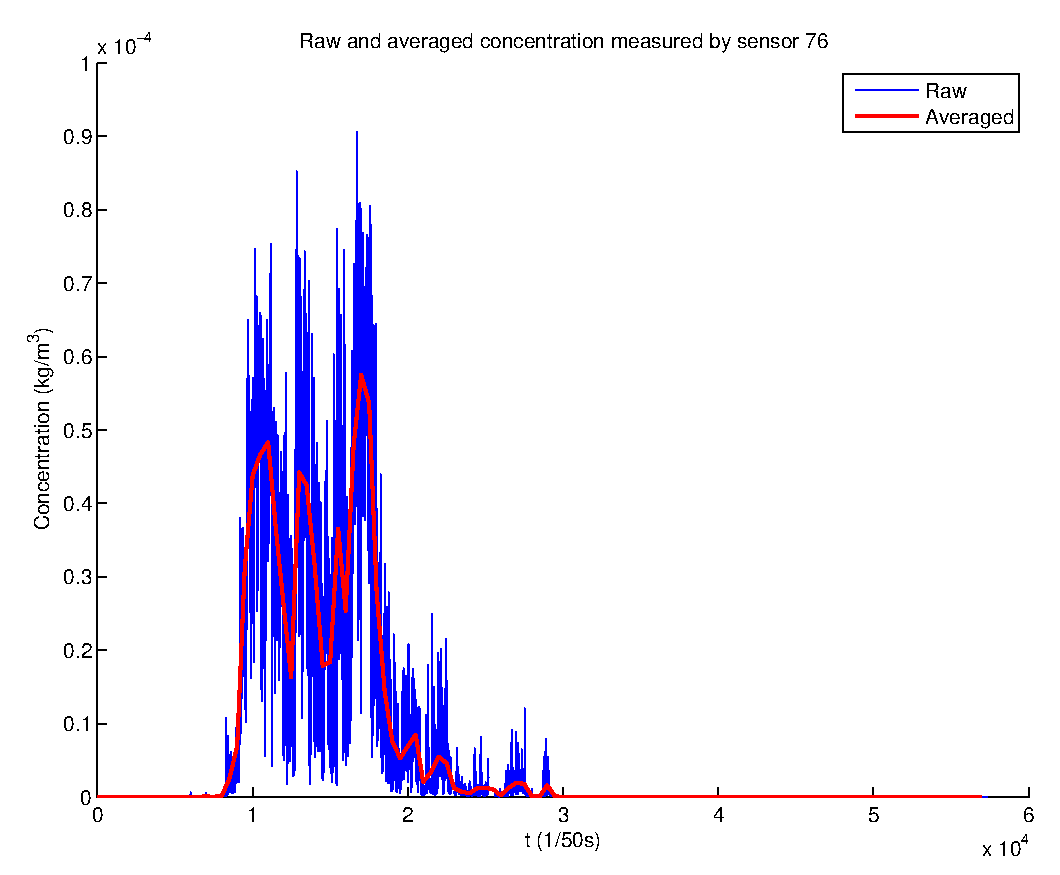
\includegraphics[scale=0.65]{moyennage_concentrations}
	\caption{Concentrations brutes (en bleu) et concentrations moyennées (en rouge) sur une fenêtre glissante de 10s. }
	\label{fig_AE_3}
\end{figure}


L'expérience FFT07 étant un outil de validation, le domaine d'étude comprend beaucoup plus de capteurs que dans un cas standard, où le domaine est moins instrumenté. Afin d'envisager un cas réaliste tout en conservant une quantité suffisante de données d'observation à traiter, nous avons choisi de limiter le nombre de capteurs {exploités} à 25 (voir figure \ref{fig_AE_4}).

\begin{figure}[h!]
	\centering
	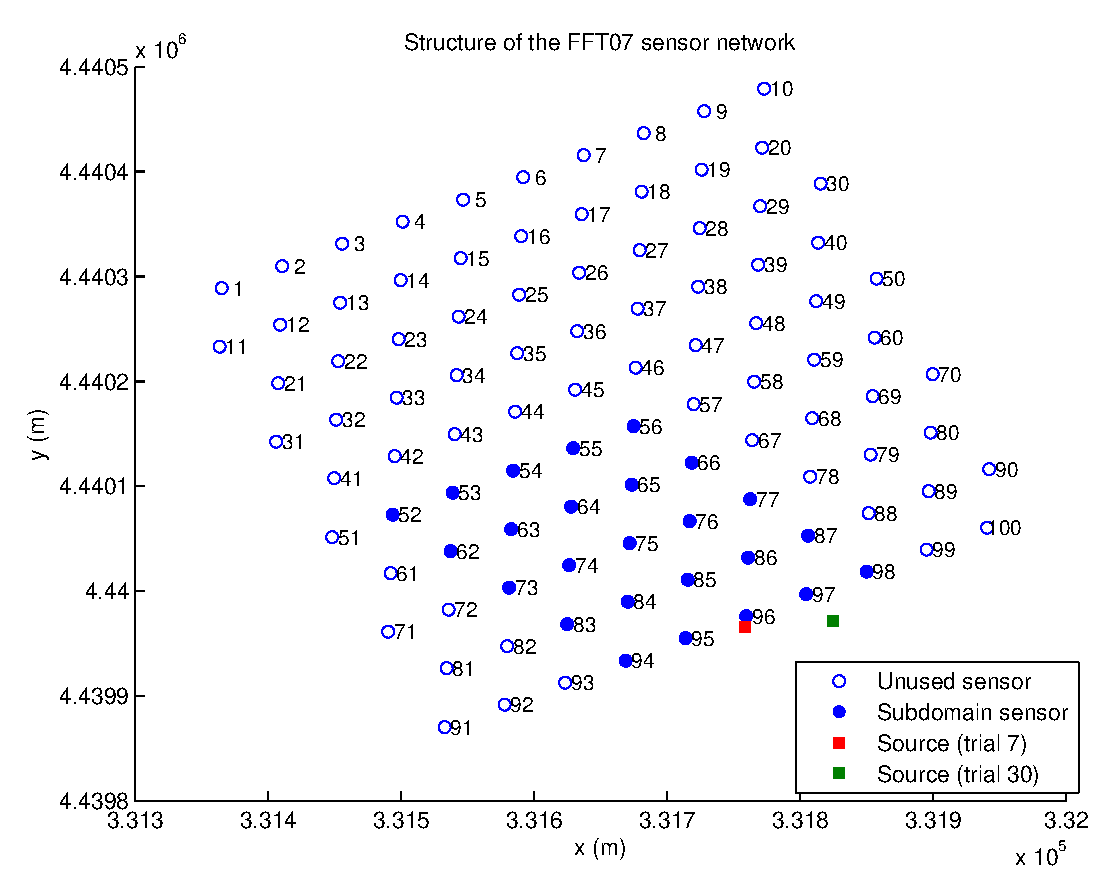
\includegraphics[scale=0.65]{FFT07_capteurs}
	\caption{Choix du sous-réseau de 25 capteurs utilisé dans notre étude.}
	\label{fig_AE_4}
\end{figure}

Dans notre cas, nous travaillons avec les configurations issues des \textit{trials} 7 et 30 {dont les données nous sont disponibles}: 
\begin{itemize}
	\item Dans un premier temps, nous simulons à l'aide d'un modèle de dispersion les concentrations mesurées aux capteurs pour chaque \textit{trial}, afin d'exclure toute source d'erreur pouvant être causée par les différents facteurs instrumentaux.
	\item Nous confrontons ensuite l'algorithme de reconstruction du terme source aux mesures réelles des capteurs, afin de vérifier si l'estimation reste suffisamment précise par rapport au cas purement synthétique.
\end{itemize}



\section{Formulation bayésienne du problème STE}

\subsection{Modèle de données et vraisemblance}

Nous considérons ici une source localisée en un point $\PosSource = (x_s, y_s, z_s)$ de l'espace et caractérisée par un profil de rejet $\VecQSource$. Pour les besoins de la modélisation, ce dernier est discrétisé en $T_s$ échéances d'émission $t'_1, \cdots, t'_{T_s}$, l'intervalle entre deux échéances consécutives demeurant strictement identique. On peut ainsi définir $\VecQSource$ comme une succession de paliers d'émissions constantes, le débit de la source ne variant pas entre deux instants d'émission consécutifs $t'_n$ et $t'_{n+1}$.\\


On suppose que les observations sont définies par des mesures de concentration en un nombre fini de points $ \PosCapteur^{(1)}, \cdots, \PosCapteur^{(N_c)}$ du domaine, qui constituent les positions d'un réseau de $N_c$ capteurs. On considère que les capteurs et la source se situent à la même hauteur, ce qui permet de n'étudier la position de la source que sur deux dimensions, autrement dit écrire $\PosSource = (x_s, y_s)$. Les mesures fournies par ces capteurs sont données suivant une discrétisation temporelle donnée, chaque capteur délivrant ainsi une valeur de concentration à chacun des instants d'observation $t_1, \cdots, t_{T_c}$.




 La concentration $\obs_{i,j}$ fournie par le $i$-ème capteur à la position $\PosCapteur^{(i)}$ et à l'échéance d'observation $t_j$ est alors modélisée par l'équation suivante: 
 
\begin{equation}
\obs_{i,j} = \sum\limits_{n=1}^{T_s}q(t'_n)\MatC_{i,j}(\PosSource, t'_n) + \varepsilon_{i,j}
\label{eq_AE_2}
\end{equation}

Le premier terme de l'équation \eqref{eq_AE_2} représente à la concentration moyenne obtenue par la superposition des $T_s$ rejets aux  différents temps d'émission $\left\{t'_n\right\}_{1\leq n \leq T_s}$et pondérés par les quantités émises $\left\{q(t'_n)\right\}_{1 \leq n \leq T_s}$ associées. Ainsi, $\MatC_{i,j}(\PosSource, t'_n)$ désigne la concentration moyenne observée par le $i$-ème capteur à la position $\PosCapteur^{(i)}$ et à l'échéance d'observation $t_j$ pour un rejet unitaire  émis à l'instant $t'_n$ par une source située à la position $\PosSource$. Enfin, $\varepsilon_{i,j}$ représente le terme regroupant toutes les sources d'erreur présentées au paragraphe §\ref{ss_erreurs}.\\

Il est possible de réécrire l'équation \eqref{eq_AE_2} sous la forme matricielle suivante:

\begin{equation}
\VecObs = \MatC(\PosSource)\VecQSource + \VecErreur
\label{eq_AE_3}
\end{equation}
qui n'est autre que l'équivalent de l'équation \eqref{eq_relation_SR_non_parametrique}. $\VecObs \in \mathbb{R}^{N_cT_c}$ est un vecteur où toutes les observations de concentration sont concaténées sous la forme suivante : 

\begin{equation}
\VecObs = \left(\obs_{1,1}, \obs_{1,2}, \cdots, \obs_{1,T_c}, \obs_{2,1}, \cdots, \cdots, \obs_{N_c,T_c}\right)^T
\label{eq_AE_3_plus}
\end{equation}

$\VecErreur \in \mathbb{R}^{N_cT_c}$ est un vecteur d'erreur qui suit, comme présenté à l'équation \eqref{eq_bruit_obs}, une loi normale centrée de matrice de covariance $\MatR \in \mathbb{R}^{N_cT_c \times N_cT_c}$. De plus, on considère que ce vecteur de bruit affecte les observations de façon indépendante et identiquement distribuée (i.i.d.): par conséquent, la matrice $\MatR$ est diagonale: 


\begin{equation}
	{
		\MatR = \varObs \MatId_{N_c T_c}
		}
\end{equation}

Le terme $\MatC(\PosSource) \in \mathbb{R}^{N_cT_c \times T_s}$ est la matrice source-récepteur suivante:

\begin{equation}
\MatC(\PosSource) = 
\begin{pmatrix}
\MatC_{1,1}(\PosSource, t'_1) & \MatC_{1,1}(\PosSource, t'_2)  & \cdots & \MatC_{1,}(\PosSource, t'_{T_s}) \\ 
\MatC_{1,2}(\PosSource, t'_1) & \MatC_{1,2}(\PosSource, t'_2)  & \cdots & \MatC_{1,2}(\PosSource, t'_{T_s}) \\
\vdots & \vdots &  & \vdots \\
\MatC_{1,T_c}(\PosSource, t'_1) & \MatC_{1,T_c}(\PosSource, t'_2)  & \cdots & \MatC_{1,T_c}(\PosSource, t'_{T_s}) \\
\MatC_{2,1}(\PosSource, t'_1) & \MatC_{2,1}(\PosSource, t'_2)  & \cdots & \MatC_{2,1}(\PosSource, t'_{T_s}) \\
\vdots & \vdots &  & \vdots \\
\vdots & \vdots &  & \vdots \\
\MatC_{N_c,T_c}(\PosSource,  t'_1) & \MatC_{N_c,T_c}(\PosSource,  t'_2)  & \cdots & \MatC_{N_c,T_c}(\PosSource,  t'_{T_s}) \\
\end{pmatrix}
\label{eq_AE_4}
\end{equation}

Si on note $\VecThetaMaj = (\PosSource, \VecQSource)$ le vecteur des paramètres caractérisant le terme source, la règle de Bayes permet {de définir} la loi a posteriori de $\VecThetaMaj$ : 

\begin{equation}
p(\VecThetaMaj | \VecObs) = \dfrac{p(\VecObs | \VecThetaMaj)p(\VecThetaMaj)}{p(\VecObs)}
\label{eq_AE_1}
\end{equation}

Comme expliqué au paragraphe \ref{paragraphe_paradigme_bayesien}, on cherche à estimer cette loi a posteriori à un facteur multiplicatif près, l'équation \eqref{eq_AE_1} devient alors:

\begin{equation}
{
p(\VecThetaMaj | \VecObs) \propto p(\VecObs | \VecThetaMaj)p(\VecThetaMaj)
}
\label{eq_AE_1_prop}
\end{equation}

Comme {le vecteur d'erreur est supposé gaussien centré}, on peut alors définir la vraisemblance des observations $\VecObs$ sachant un terme source donné $\VecThetaMaj$:

\begin{equation}
p(\VecObs | \VecThetaMaj) = \prod\limits_{i=1}^{N_c} \prod\limits_{j=1}^{T_c}\mathcal{N}\left(\obs_{i,j} \middle\vert \MatC_{i,j}(\PosSource)\VecQSource, \varObs\right)
\label{eq_AE_5}
\end{equation}

\subsection{Choix des lois a priori}

\subsubsection{Position de la source}

On considère que la source est forcément contenue dans les limites du domaine spatial $\mathcal{D}$ considéré, mais qu'elle peut se situer en n'importe quel point de ce domaine. En termes probabilistes, cela se traduit par une loi a priori uniforme sur la position $\PosSource$ de la source:

\begin{equation}
p(\PosSource) = \mathcal{U}_\mathcal{D}(\PosSource)
\label{eq_AE_7}
\end{equation}


\subsubsection{Profil d'émission}

Comme expliqué dans \cite{Winiarek2011}, la pratique la plus courante consiste à choisir un a priori gaussien pour le vecteur $\VecQSource$, qui s'écrit alors:

\begin{equation}
p(\VecQSource) = \mathcal{N}\left(\VecQSource \middle \vert \VecMeanQ, \MatCovQ\right)
\label{eq_AE_8}
\end{equation}

Dans \cite{Bocquet2008}, il est expliqué que l'hypothèse gaussienne sur $\VecQSource$ entraîne potentiellement des incohérences physiques telles que des valeurs d'émissions négatives. Cependant, une telle hypothèse demeure fréquemment utilisée dans la littérature, et conduit à des résultats satisfaisants (voir par exemple \cite{Issartel2003}) ainsi qu'une meilleure flexibilité quant à la quantification des connaissances a priori sur le type de rejet étudié. Par exemple, si on sait d'avance que le rejet se fait à un débit relativement faible, alors il est possible d'ajuster les valeurs de la diagonale de la matrice de covariance en y mettant des quantités faibles. \\

Il est toutefois possible d'atténuer les effets indésirables de l'hypothèse gaussienne sans avoir à changer la nature de la loi de probabilité a priori de $\VecQSource$, nous verrons comment cela est possible dans le prochain paragraphe.

\section{Démarche de résolution du problème bayésien}

\NdFS{Nous développons ici en détail le processus de résolution du problème tel qu'il a été défini dans le paragraphe précédent, à savoir \textit{le calcul de la loi a posteriori $p(\VecThetaMaj | \VecObs)$ des paramètres de la source}. En pratique, il est impossible d'obtenir cette dernière de façon analytique, à cause de la complexité et de l'aspect fortement non-linéaire de la vraisemblance $p(\VecObs|\VecThetaMaj)$ présentée à l'équation \eqref{eq_AE_5}. Afin de contourner ce problème, une solution consiste à décomposer notre loi cible en plusieurs éléments distincts, en suivant une opération de \textit{marginalisation}}.\\


\NdFS{La loi $p(\VecThetaMaj|\VecObs)$ est dite \textit{jointe}, car elle regroupe tous les paramètres de la source autour d'une unique loi a posteriori. Par définition des probabilités conditionnelles, cette loi peut s'écrire de la façon suivante:}

\begin{equation}
p(\VecThetaMaj|\VecObs) = p(\PosSource, \VecQSource | \VecObs) = \dfrac{p(\PosSource, \VecQSource, \VecObs)}{p(\VecObs)}
\label{eq_conditionalite}
\end{equation}

En appliquant la règle du conditionnement en chaîne, ou \textit{chain rule}\footnote{La \textit{chain rule} permet d'exprimer une loi jointe sous la forme d'un produit de lois conditionnelles. Si on considère les $n$ variables aléatoires $X_1, \dots, X_n$, alors on a $p(X_1, \dots, X_n) = p(X_n|X_1, \dots, X_{n-1})p(X_{n-1}|X_1, \dots, X_{n-2})\dots p(X_2|X_1)p(X_1)$.}, sur le numérateur, on arrive à l'expression suivante:
\begin{equation}
p(\PosSource, \VecQSource | \VecObs) = p(\VecQSource | \PosSource, \VecObs)p(\PosSource | \VecObs)
\label{eq_AE_9}
\end{equation}
où: 
	
	\begin{itemize}
		\item $p(\VecQSource | \PosSource, \VecObs)$ est la loi a posteriori conditionnelle de $\VecQSource$,
		\item $p(\PosSource | \VecObs)$ est la loi a posteriori marginale de $\PosSource$.
	\end{itemize} 

\subsection{Loi conditionnelle du profil d'émission}

\subsubsection{A priori gaussien et solution analytique}


{
	Etant donnés les paramètres $\VecMeanQ$ et $\MatSigma_q$ définis à l'équation \eqref{eq_AE_8} et la formulation du modèle de l'équation \eqref{eq_AE_3}  il est possible de réécrire la vraisemblance sous la forme suivante:
	
	\begin{equation}
		p(\VecObs | \VecQSource, \PosSource) = \mathcal{N}(\VecObs | \MatC(\PosSource)\VecMeanQ, \MatC(\PosSource)\MatSigma_q\MatC(\PosSource)^T + \MatR)
		\label{eq_lk_gaussian}
	\end{equation}
	
	La loi a priori de $\VecQSource$ ainsi que la vraisemblance de l'équation \eqref{eq_lk_gaussian} suivant toutes deux des lois normales, alors la loi a posteriori \NdFS{conditionnelle} de $\VecQSource$ suit également une loi normale de moyenne $\PostMeanQ$ et de matrice de covariance $\PostCovQ$, dont les valeurs sont obtenues par les formules empiriques: 
	 \begin{equation}
	 \begin{split}
	 \PostMeanQ (\VecPosSource) & = \VecMeanQ + \MatK(\VecObs - \MatC(\PosSource)\VecMeanQ) \\
	 \PostCovQ (\VecPosSource) & = \MatCovQ - \MatK\MatC(\PosSource)\MatCovQ
	 \end{split}
	 \label{eq_filtre_kalman_statique}
	 \end{equation}
	  où $\MatK$ est définie par:
	  
	  \begin{equation}
	  \MatK = \MatCovQ\MatC(\PosSource)^T(\MatC(\PosSource)\MatCovQ\MatC(\PosSource)^T + \MatR)^{-1}
	  \end{equation}
	
	}
  \NdFS{Pour une valeur de $\VecPosSource$ donnée, les paramètres $\PostMeanQ(\VecPosSource)$ et $\PostCovQ(\VecPosSource)$ sont ainsi obtenus de façon analytique (i.e. sans approximation) par les équations \eqref{eq_filtre_kalman_statique}. Dans un souci de lisibilité, on notera plus simplement $\PostMeanQ$ et $\PostCovQ$ par la suite.}

\subsubsection{Contrainte de positivité}

Dans le but d'assurer la positivité des valeurs d'émission de la source, une contrainte peut être appliquée sur les résultats de l'équation \eqref{eq_filtre_kalman_statique}, inspirée par les travaux de \cite{Simon2010}. Il s'agit d'utiliser une méthode permettant de restreindre les valeurs d'un vecteur d'état à un intervalle borné ou semi-borné prédéfini: pour cela, la densité de probabilité de ce vecteur d'état est tronquée suivant la contrainte que l'on cherche à appliquer. \\

Le processus de troncature est ainsi appliqué de façon séquentielle sur chaque composante de $\VecQSource$: on travaille ainsi à tronquer $T_s$ densités de loi univariées. Le détail de cette démarche est décrit par l'algorithme \ref{algo_PCO}, qui permet d'approximer la loi a posteriori \NdFS{conditionnelle} de $\VecQSource$ par : 

\begin{equation}
p^c(\VecQSource | \PosSource, \VecObs) = \mathcal{N}(\VecQSource | \PostMeanQ^c, \PostCovQ^c)
\label{eq_AE_16}
\end{equation}

\begin{algorithm}
\begin{algorithmic}
	\State \textbf{Entrées}: $\PostMeanQ$ et $\PostCovQ$
	\State Initialisation: $\PostMeanQ^c=\PostMeanQ$ et $\PostCovQ^c=\PostCovQ$
	\For{$i=1:T_s$}
		\State ${\bm \gamma}_i=\begin{bmatrix}{\bf 0}_{1\times (i-1)} & 1  & {\bf 0}_{1\times (T_s-i)}\end{bmatrix}^T$
		\State Calculer ${\bm W}_i$ et ${\bm T}_i$ par la réduction de Jordan de $\PostCovQ^c$, i.e. ${\bm T}_i {\bm W}_i {\bm T}_i^T=\PostCovQ^c$
		\State Calculer ${\bm S}_i$ par l'orthogonalisation de Gram-Schmidt pour obtenir la matrice orthogonale ${\bm S}_i$ telle que $${\bm S}_i {\bm W}_i^{1/2} {\bm T}_i^T {\bm \gamma}_i=\begin{bmatrix}
		({\bm \gamma}_i^T \PostCovQ^c {\bm \gamma}_i)^{1/2} & 0 & \cdots & 0 
		\end{bmatrix} $$
		 $c_i=-\dfrac{{\bm \gamma}_i^T \PostMeanQ^c}{({\bm \gamma}_i^T \PostCovQ^c {\bm \gamma}_i)^{1/2}}$
		 \State $\mu_i=\dfrac{\phi(c_i)}{1-\Phi(c_i)}$ avec $\phi(\cdot)$ la densité de la loi normale centrée réduite, et $\Phi(\cdot)$ la fonction de répartition de la loi normale centreé réduite.
		 \State $\sigma^2_i=1-\mu_i(\mu_i-c_i)$
		 \State ${\bm z}_i=\begin{bmatrix}\mu_i & 0 & \cdots & 0 \end{bmatrix}^T$
		 \State ${\bm D}_i=\text{diag}(\sigma^2_i,1,\ldots,1)$
		\State Calculer les paramètres de la densité tronquée:
		\State \begin{align*}
		\begin{split}
		\PostMeanQ^c&={\bm T}_i {\bm W}_i^{1/2} {\bm S}_i ^T{\bm z}_i + \PostMeanQ^c\\
		\PostCovQ^c&={\bm T}_i {\bm W}_i^{1/2} {\bm S}_i^T {\bm D}_i  {\bm S}_i {\bm W}_i^{1/2} {\bm T}_i ^T \\
		\end{split}
		\end{align*}
	\EndFor
	\State \textbf{Sorties}: $\PostMeanQ^c$ et $\PostCovQ^c$
	\end{algorithmic}
	\caption{Contrainte de positivité sur $\VecQSource$ par troncature de la densité de $p(\VecQSource | \PosSource, \VecObs)$}
	\label{algo_PCO}
\end{algorithm}

Notons qu'une telle procédure permet également d'optimiser le calcul de la vraisemblance marginale de la localisation de la source $p(\VecObs | \PosSource)$: celle-ci peut alors se calculer par le même procédé que celui employé dans l'équation \eqref{eq_AE_9}, et devient alors:

\begin{equation}
p^c(\VecObs | \PosSource) = \dfrac{p(\VecObs | \VecQSource, \PosSource)p(\VecQSource)}{p^c(\VecQSource | \PosSource, \VecObs)}
\label{eq_AE_17}
\end{equation}


 \begin{figure}[h!]
 	\centering
 	\begin{subfigure}[t]{0.5\textwidth}
 		\centering
		\includegraphics[width=1\textwidth]{ConstrainedFigure1.eps}
		\caption{}
 		\label{fig_AE_2_a}
 	\end{subfigure}%
 	\begin{subfigure}[t]{0.5\textwidth}
 		\centering
		\includegraphics[width=1\textwidth]{ConstrainedFigure2.eps}
		\caption{}
 		\label{fig_AE_2_b}
 	\end{subfigure}
 	\begin{subfigure}[t]{0.5\textwidth}
 		\centering
 		\includegraphics[width=1\textwidth]{ConstrainedFigure3.eps}
 		\caption{}
 		\label{fig_AE_2_c}
 	\end{subfigure} 

 	\caption{Illustration de l'application de la contrainte de positivité (en noir) sur les paramètres d'une distribution gaussienne bivariée (en rouge) dans trois cas distincts: sans corrélation (\ref{fig_AE_2_a}), avec corrélation négative (\ref{fig_AE_2_b}) et avec corrélation positive (\ref{fig_AE_2_c}).}
 	 \label{fig_AE_2}	
 \end{figure}

La figure \ref{fig_AE_2} résume bien le fonctionnement de l'algorithme \ref{algo_PCO}: la zone en noir représente la version tronquée aux valeurs positives de la distribution initiale (en rouge). 

\subsection{Localisation de la source avec l'algorithme AMIS}

Il s'agit ici d'étudier la loi a posteriori marginale $p(\PosSource | \VecObs)$ de la position de la source. Contrairement au profil d'émission, il est {impossible} d'obtenir une solution analytique pour caractériser cette distribution. Par conséquent, {l'idée est d'utiliser les méthodes de simulation stochastique afin d'}approximer la distribution $p(\PosSource | \VecObs)$. \\

\subsubsection{Principe}

Nous appliquons l'algorithme AMIS décrit dans le chapitre 2 afin de localiser la source. Pour cela, on va ainsi construire une procédure itérative basée sur l'algorithme \ref{algo_AMIS} afin de créer sur $K$ itérations et en générant $N_p$ particules par itération un échantillon de $KN_p$ particules {$\left\{\PosSource_k^{(i)}\right\}_{0\leq k \leq K}^{1\leq i \leq N_p}$} dont la distribution approxime celle de la loi marginale a posteriori {$p(\PosSource | \VecObs)$} de la position de la source.\\

Dans un cadre bayésien, la loi cible recherchée peut alors s'écrire à une constante multiplicative près, suivant la relation de proportionnalité suivante:

\begin{equation}
{
p(\PosSource | \VecObs) \propto p(\VecObs | \PosSource)p(\PosSource)
\label{eq_AE_20}
}
\end{equation}

La fonction de vraisemblance {$p(\VecObs | \PosSource)$} est définie par l'équation \eqref{eq_AE_5} (ou \eqref{eq_AE_17} si on choisit d'appliquer la contrainte de positivité), et la loi a priori {$p(\PosSource)$} par l'équation \eqref{eq_AE_7}. L'équation \eqref{eq_AE_20} permet ainsi d'évaluer la loi cible toute particule {$\PosSource$} échantillonnée depuis la loi de proposition courante, afin de calculer les poids d'importance {associés}. La structure globale de la démarche est décrite par la figure \ref{schema_amis}.\\

%\begin{figure}[h!]
%	\centering
%	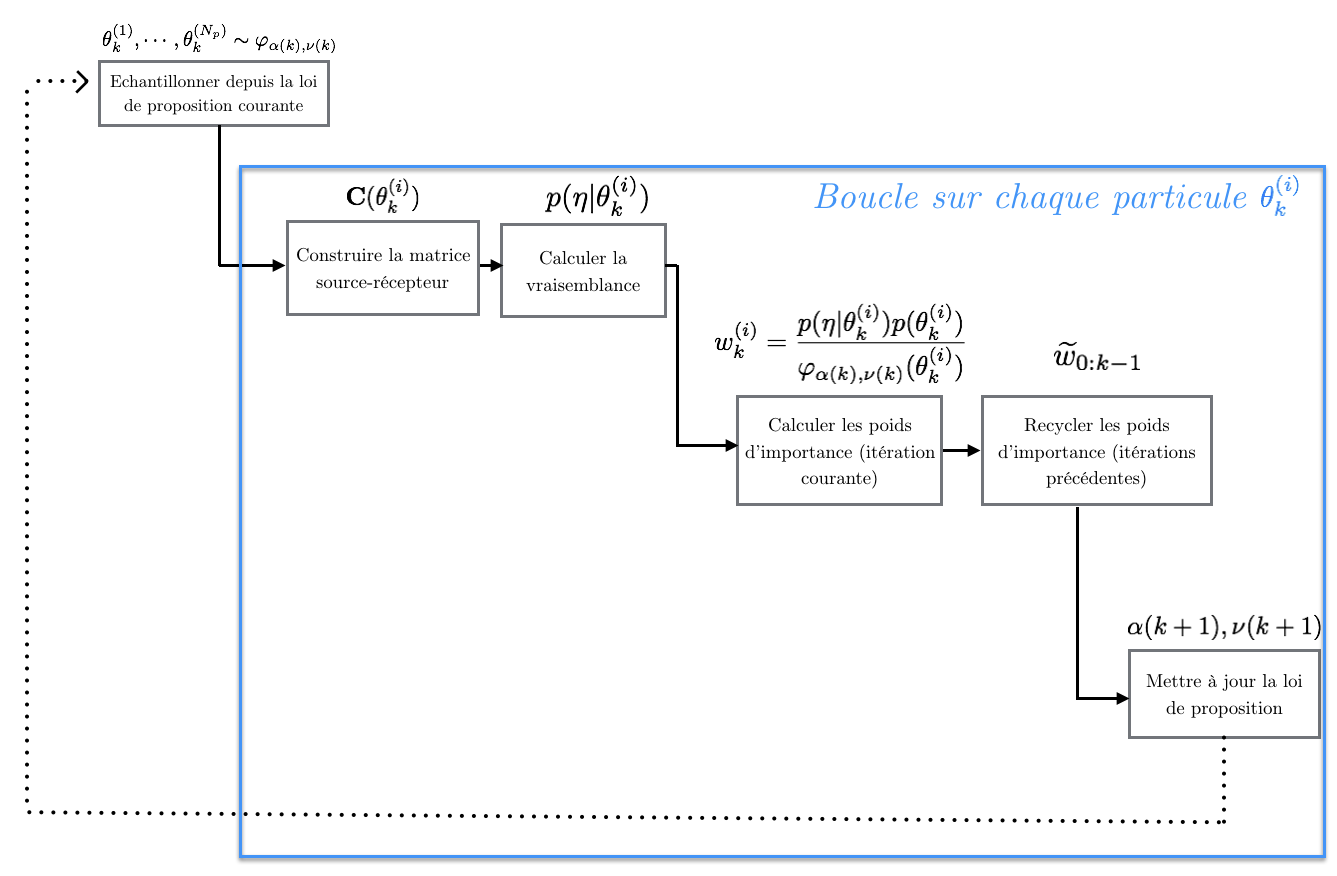
\includegraphics[width=1\textwidth]{schema_amis_capture}

%\end{figure}
\begin{figure} 
		\centering
        \begin{tikzpicture}[retour/.style={->,>=stealth’,thick,dashed}]
        \node[draw, text width = 7cm, align=center] (step_1) at (0,0) {Echantillonner $\PosSource_k^{(1)}, \dots, \PosSource_k^{(N_p)}$  depuis la loi de proposition courante $\varphi_{\alpha(k), \nu(k)}$};
        \node[draw, text width = 7cm, align=center] (step_2) at (0,-1.75) {Construire les matrices source-récepteur $\MatC(\PosSource_k^{(1)}), \dots, \MatC(\PosSource_k^{(N_p)})$ avec $N_p$ \\appels au modèle de dispersion direct};
        \node[draw, text width = 7cm, align=center] (step_3) at (0,-3.5) {Calculer les vraisemblances \\ $p(\VecObs | \PosSource_k^{(1)}), \dots, p(\VecObs | \PosSource_k^{(N_p)})$};
        \node[draw, text width = 7cm, align=center] (step_4) at (0,-6.5) {Pour chaque $i \in \{1, \cdots, N_p\}$, calculer les poids d'importance \\ $ w_k^{(i)} = \dfrac{p(\VecObs | \PosSource_k^{(i)})p(\PosSource_k^{(i)})}{\varphi_{\alpha(k), \nu(k)}(\PosSource_k^{(i)})}$ \\et normaliser: \\$\widetilde{w}_k^{(i)} = \dfrac{w_k^{(i)}}{\sum\limits_{j=1}^{N_p} w_k^{(j)}}$};
        \node[draw, text width = 7cm, align=center] (step_5) at (0,-9.75) {Recycler les poids d'importance des itérations précédentes \\ $\widetilde{w}_l^{(1)}, \dots, \widetilde{w}_l^{(N_p)}$ avec $l \in \{0, \dots, k-1\}$}; 
        \node[draw, text width = 7cm, align=center] (step_6) at (0,-12) {En utilisant $\PosSource_l^{(1)}, \dots, \PosSource_l^{(N_p)}$ et $\widetilde{w}_l^{(1)}, \dots, \widetilde{w}_l^{(N_p)}$ avec $l \in \{0, \dots, k\}$, générer les nouveaux paramètres \\ $\alpha(k+1)$ et $\nu(k+1)$ de la loi de proposition };
        %\draw[retour] (step_6)--(step_1);
        \draw[->,>=latex] (step_1) -- (step_2);
        \draw[->,>=latex] (step_2) -- (step_3);
        \draw[->,>=latex] (step_3) -- (step_4);
        \draw[->,>=latex] (step_4) -- (step_5);
        \draw[->,>=latex] (step_5) -- (step_6);
        \end{tikzpicture}
        \caption{Diagramme de fonctionnement de l'algorithme AMIS sur la $k$-ième itération pour la localisation de la source.}
        \label{schema_amis}
 \end{figure}

\subsubsection{Choix de la loi de proposition}

L'algorithme AMIS requiert une loi de proposition paramétrique qui soit suffisamment flexible pour:
{
	\begin{itemize}
		\item pouvoir s'adapter de façon à être capable d'approximer correctement la loi cible une fois ses paramètres ajustés,
		\item effectuer simplement l'opération d'adaptation des paramètres. Sur ce point, le choix d'une mixture de gaussiennes telle que présentée dans \cite{Cappe2008} est cohérent, car les formules de mise à jour sont directement disponibles via l'algorithme EM.
	\end{itemize}

On définit donc la loi de proposition comme} une mixture de $D$ distribution gaussiennes bivariées:

\begin{equation}
\varphi_{(\alpha,\nu)}({\PosSource}) = \sum\limits_{d=1}^D \alpha_d \varphi_d({\PosSource} | \nu_d)
\label{eq_AE_21}
\end{equation}
où les $\alpha_d$ sont les facteurs d'influence de chacune des composantes de la mixture, et $\nu_d$ représente le vecteur des paramètres de la $d$-ième composante, telle que : 
\begin{equation}
\varphi_d({\PosSource} | \nu_d) = \mathcal{N}({\PosSource} | \VecMu_d, \MatSigma_d)
\label{eq_AE_21_bis}
\end{equation}
avec $\VecMu_d \in \mathbb{R}^2$ et $\MatSigma_d \in \mathbb{R}^{2\times2}$.

 \begin{figure}[h!]
 	\centering
 	\begin{subfigure}[t]{0.5\textwidth}
 		\centering
 		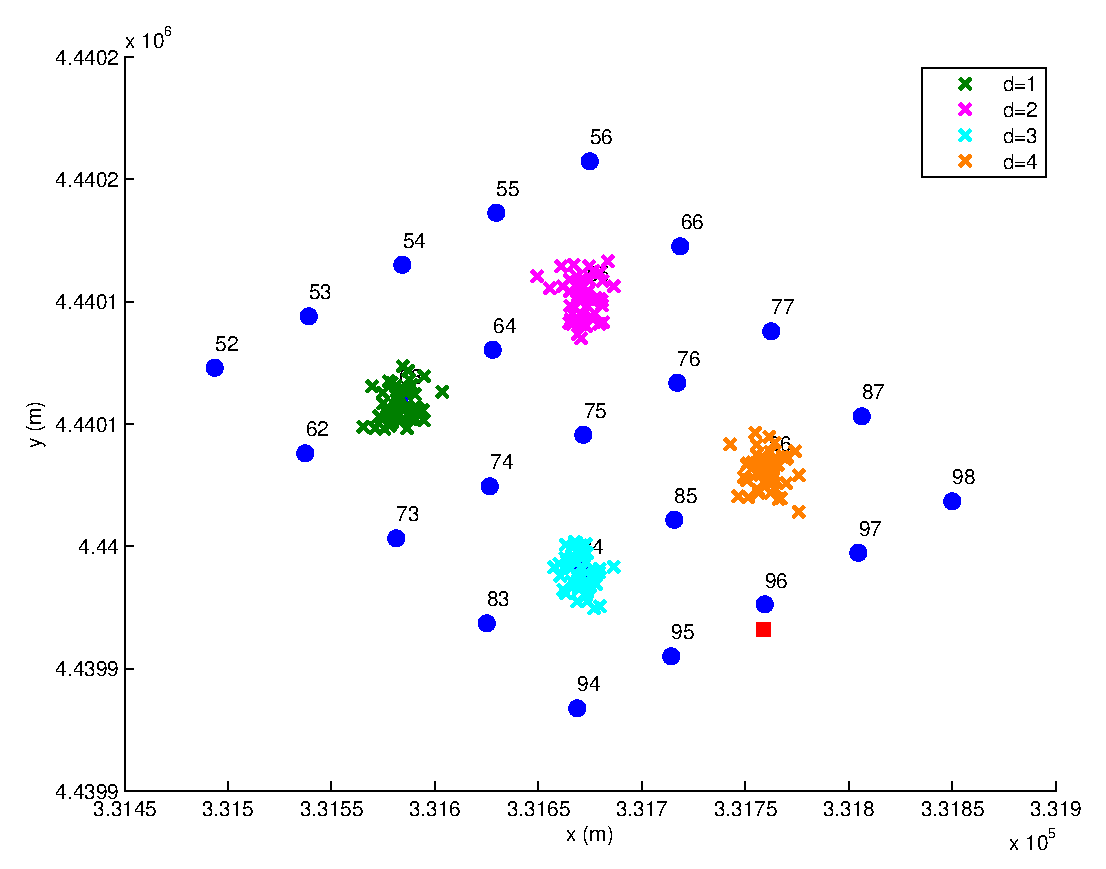
\includegraphics[width=1\textwidth]{init_amis_bad.eps}
 		\caption{$\MatSigma_d = 
 			\begin{pmatrix}
 			50 & 0 \\
 			0 & 50
 			\end{pmatrix}$}
 		\label{init_amis_bad}
 	\end{subfigure}%
 	\begin{subfigure}[t]{0.5\textwidth}
 		\centering
 		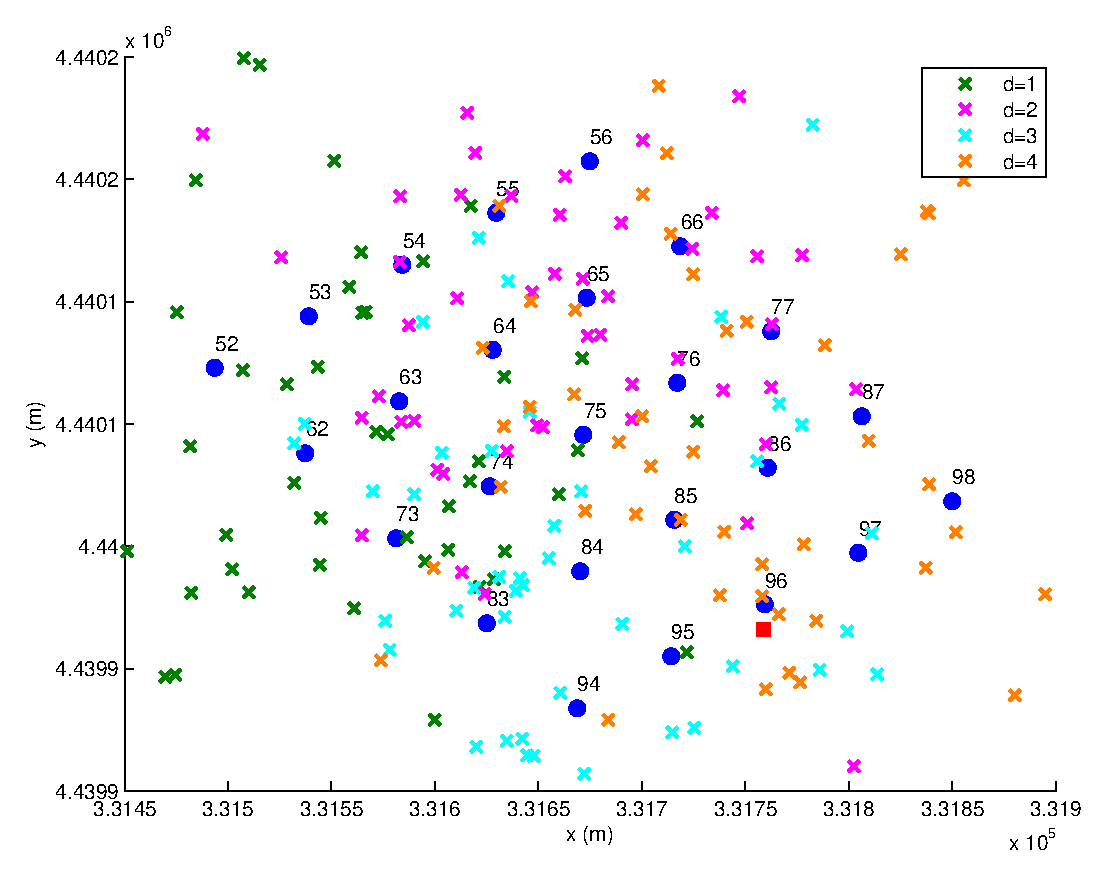
\includegraphics[width=1\textwidth]{init_amis_good.eps}
 		\caption{$\MatSigma_d = 
 			\begin{pmatrix}
 			5000 & 0 \\
 			0 & 5000
 			\end{pmatrix}$}
 		\label{init_amis_good}
 	\end{subfigure}
 	\caption{Exemples d'initialisation de l'AMIS avec $D=4$ composantes pour la loi de proposition: un bon choix des $\MatSigma_d$ permet un tirage homogène sur le domaine (\ref{init_amis_good}) tandis qu'une covariance trop faible ne permettra pas d'explorer tout le domaine (\ref{init_amis_bad}).}
 	 \label{fig_init_amis}	
 \end{figure}
 
  Le choix des paramètres initiaux permet de régler la surface couverte par chacune des composantes afin d'obtenir une répartition relativement homogène des particules, illustrant une absence de connaissance a priori sur une localisation potentielle de la source (voir figure \ref{fig_init_amis}). \\
  
  En pratique, nous avons:
  
  \begin{enumerate}
  	\item divisé le domaine en quatre quadrants de surface égale, 
  	\item  placé les moyennes $\VecMu_d$ sur le centre de chacun des quadrants,
  	\item réglé les matrices de covariance $\MatSigma_d$ de façon à ce que chacune des composantes de la mixture fournisse des échantillons couvrant toute la surface de son quadrant.\\
  \end{enumerate}
  
 {Si une information a priori est disponible (par exemple, des zones particulières du domaine à exclure ou à favoriser), les paramètres $\alpha_d, \VecMu_d$ et $\MatSigma_d$ avec $d \in \{1,\dots,D\}$ peuvent être préalablement ajustés afin d'orienter en conséquence l'échantillonnage des particules dès la première itération. Un exemple de ce type d'initialisation est présenté au Chapitre 4.
 	
 	Une fois l'algorithme lancé, à chaque itération, ces paramètres  sont mis à jour grâce aux formules des équations \eqref{eq_maj_gaussien}.}\\

\subsection{Loi a posteriori jointe des paramètres de la source}



\NdFS{En suivant la procédure décrite par l'algorithme \ref{schema_amis} sur un total de $K$ itérations, la loi a posteriori marginale de la position de la source peut être approximée grâce à \eqref{eq_IS_poids_normalises} de la façon suivante:
	
\begin{equation}
	p(\VecPosSource | \VecObs) \simeq \sum\limits_{k=1}^K \sum\limits_{i=1}^{N_p} \widetilde{w}_k^{(i)} \VecPosSource_k^{(i)} \delta_{\VecPosSource_k^{(i)}} d\VecPosSource
	\label{eq_marginal_posterior_location}
\end{equation}

En reprenant l'expression  de la loi a posteriori jointe \eqref{eq_AE_9}, on obtient finalement la solution suivante:

 \begin{equation}
p(\VecPosSource, \VecQSource | \VecObs) \simeq \sum\limits_{k=1}^K \sum\limits_{i=1}^{N_p} \widetilde{w}_k^{(i)} p(\VecQSource | {\VecPosSource}_k^{(i)}, \VecObs) \delta_{{\VecPosSource}_k^{(i)}} d\VecPosSource
 \label{eq_joint_posterior}
 \end{equation}

Afin d'interpréter les résultats de localisation de la source, on peut estimer la densité a posteriori via une approche de type KDE en utilisant les échantillons tirés via l'AMIS. Pour une estimation ponctuelle, on peut avoir recours au MMSE. \\

Pour obtenir une estimation du profil d'émission de type MMSE, on moyenne les valeurs de $\PostMeanQ$ obtenues pour chaque particule échantillonnée par l'AMIS en respectant la pondération imposée par les poids d'importance correspondants. \\

Ces différents modes d'interprétation sont utilisés dans le paragraphe relatifs aux résultats obtenus sur la campagne FFT07.\\

}

\section{Description du modèle de dispersion à bouffées gaussiennes}

Une fois la loi de proposition initialisée, on peut exécuter la boucle itérative de l'algorithme AMIS telle que décrite à l'algorithme \ref{algo_AMIS}. Dans cet algorithme, le calcul de la loi de vraisemblance telle que décrite à l'équation \eqref{eq_AE_5} requiert l'exécution d'un modèle de dispersion pour obtenir $\MatC(\PosSource)$. Ici, nous choisissons d'utiliser un modèle \textit{à boufféees gaussiennes}, ou \textit{Gaussian Puff Model} (GPM). Nous expliquons brièvement dans la suite de ce paragraphe les principes de base régissant ce type de modèles.\\

Les modèles gaussiens permettent de représenter la dispersion à petite échelle autour d'une source. Pour cela, une formulation analytique de la concentration du polluant est calculée suivant plusieurs hypothèses permettant une mise en oeuvre simple et peu coûteuse en temps de calcul. Il existe deux types différents de modèles gaussiens:\\

\begin{itemize}
	\item les modèles dits \textit{de panache} (ou \textit{Gaussian plume}), où la dispersion est modélisée dans des conditions météorologiques supposées uniformes et stationnaires. Le panache émis par la source est alors modélisé par une distribution de type gaussienne dans deux directions: celle orthogonale au vent, et la direction verticale (voir figure \ref{gaussian_plume}).
	\item les modèles dits \textit{à bouffées} (ou \textit{Gaussian puff}), modélisant une série d'émissions instantanées représentées par des bouffées à distribution gaussienne dans les trois directions de l'espace, et dont les centres sont transportés par un champ de vent qui peut  être non-uniforme et non-stationnaire. La globalité du rejet à un instant donné est ainsi illustrée par la somme des différentes bouffées émises par la source (voir figure \ref{gaussian_puff}). C'est ce type de modèle que nous utilisons dans l'étude de cas sur FFT07.
\end{itemize}

 \begin{figure}[h!]
 	\label{fig_gaussian_models}	
 	\centering
 	\begin{subfigure}[t]{0.5\textwidth}
 		\centering
 		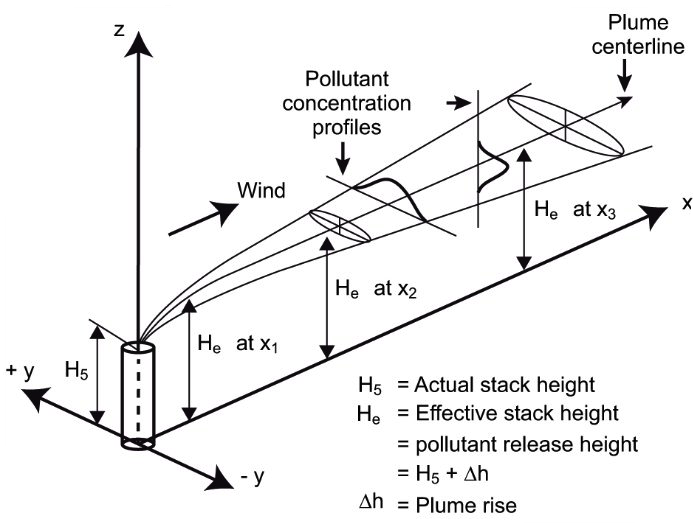
\includegraphics[width=1\textwidth]{gaussian_plume.jpg}
 		\caption{Modèle de panache gaussien \cite{Schulze1996}}
 		\label{gaussian_plume}
 	\end{subfigure}%
 	\begin{subfigure}[t]{0.5\textwidth}
 		\centering
 		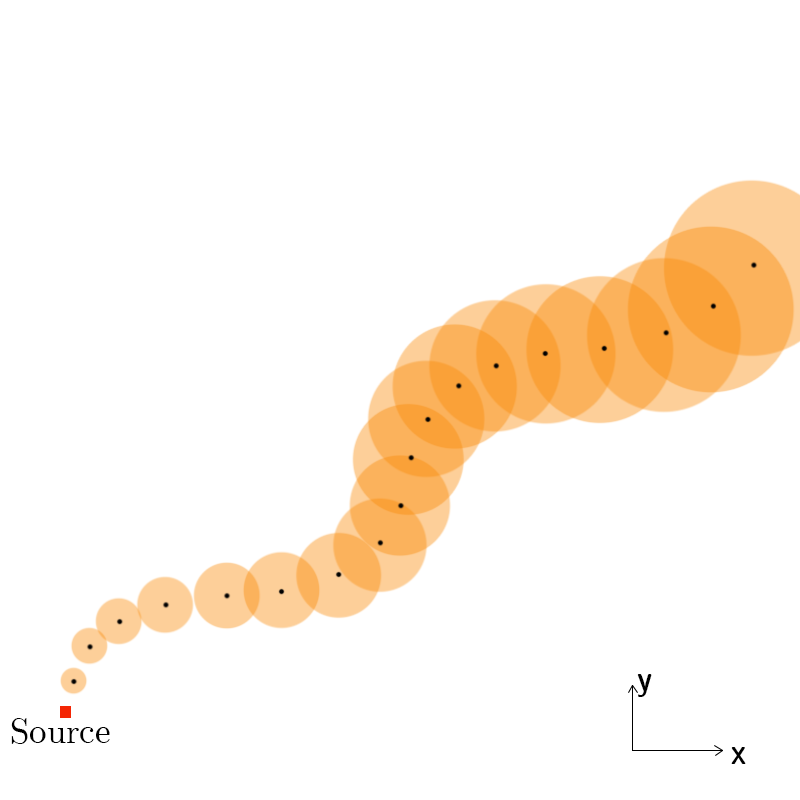
\includegraphics[width=1\textwidth]{gaussian_puff}
 		\caption{Modèle de bouffées gaussiennes}
 		\label{gaussian_puff}
 	\end{subfigure}
 	
 	\caption{Schémas de principe des modèles de dispersion gaussiens à panache (\ref{gaussian_plume}) et à bouffées (\ref{gaussian_puff})}
 \end{figure}
 
 Dans le cadre de FFT07, le choix d'un modèle à bouffées par rapport à un modèle à panache est justifié par {le caractère instationnaire} du profil d'émission que nous cherchons à estimer. La grandeur $\VecQSource$ est en effet un vecteur, et non une valeur constante, comme c'est le cas si on appliquait un modèle de type \textit{Gaussian plume}. Cela permet également de prendre en compte les variations météorologiques telles que des changements de direction de vent. \\
 
 La concentration mesurée au $i$-ème capteur $\PosCapteur^{(i)} = (x_c^{(i)}, y_c^{(i)})$ au temps d'observation $t_j$ résultant d'une source localisée en $\PosSource$ émettant un rejet instantané à l'instant $t'_n$ est donnée par: 
 
 \begin{equation}
 \MatC_{i,j}(\PosSource, t'_n) = \dfrac{2Q_u\Delta t_p}{(2\pi)^{3/2}s_x s_y s_z}\exp\left[-\dfrac{1}{2}(\Lambda_x^2 + \Lambda_y^2)\right]
 \label{eq_AE_27}
 \end{equation}
 où:
 \begin{itemize}
 	\item $Q_u$ est la quantité unitaire de polluant émise: comme les concentrations fournies par les capteurs sont en kg/m$^3$ on a $Q_u = 1\text{kg/s}$,
 	\item $\Delta t_p$ est l'écart temporel entre l'émission de deux bouffées consécutives dans le modèle de dispersion, ici $\Delta t_p = 1$s,
 	\item $s_x, s_y, s_z$ sont les coefficients de dispersion sur les trois axes de l'espace,
 	\item les grandeurs $\Lambda_x$ et $\Lambda_y$ sont définies par : 
 	
 	\begin{equation}
 	\begin{split}
 	\Lambda_x &= \dfrac{x_c^{(i)} - \left(\PosSource + \sum\limits_{t=t'_n}^{t_j}u_x(t)\delta_w\right)}{s_x}\\
 	 	\Lambda_y &= \dfrac{y_c^{(i)} - \left(\PosSource + \sum\limits_{t=t'_n}^{t_j}v_x(t)\delta_w\right)}{s_y}
 	\end{split}
 	\end{equation}
 	$\delta_w$ est l'intervalle de temps entre deux valeurs de mesures du vent, ce dernier étant représenté par ses deux composantes $u_x$ et $v_x$.
 \end{itemize}
 
 On se place dans le cas d'une diffusion isotrope en $x$ et $y$, on a ainsi $s_x = s_y$. Les valeurs de $s_y$ et $s_z$ sont obtenues par la formule suivante : 
 
 \begin{equation}
 \begin{split}
 s_y &= a_y [d(\PosSource, \bm{x}_p)]^{b_y}\\
 s_z &= a_z [d(\PosSource, \bm{x}_p)]^{b_z}
 \end{split}
 \end{equation}
 où $a_x, a_y, b_x, b_y$ sont des coefficients empiriques qui dépendent de la classe de stabilité atmosphérique \cite{Pasquill1983} et $d(\PosSource, \bm{x}_p)$ est la distance entre la source $\PosSource$ et le centre $\bm{x}_p$ de la bouffée courante. On utilise ici la classe de Pasquill D, qui est la plus appropriée pour des conditions stables en topographie non-urbaine. 
 Comme les valeurs de la composante verticale du vent qui ont été relevées sont relativement faibles, et étant donné que les capteurs et la source se trouvent assez près du sol (2m), on ne tient pas non plus compte du terme en $z$ qui apparaît dans l'exponentielle dans la formulation générale du modèle {à bouffées gaussiennes}.

\section{Présentation des résultats}

\subsection{Résultats obtenus avec des données simulées}
\label{par_simule}

Dans un premier temps, afin de valider la méthode, le choix est fait de se placer dans un cadre synthétique, à savoir reproduire les conditions de l'expérience FFT07 et simuler les concentrations mesurées aux capteurs grâce à l'exécution d'un modèle de dispersion, en l'occurence le modèle gaussien défini au paragraphe précédent. Ainsi, les positions des capteurs et des sources sont exactement les mêmes que celles des \textit{trials} 7 et 30 de FFT07. Les données météorologiques sont ajustées afin que les concentrations simulées soient les plus proches possibles des relevés expérimentaux, et le vent est considéré constant en direction et en vitesse. \\

L'algorithme AMIS a été exécuté sur $K = 10$ itérations, avec $N_p = 100$ particules échantillonnées par itération. {La loi de proposition comporte $D=4$ composantes.} Les observations synthétiques ont été générées avec un ajout de bruit gaussien centré de variance $10^{-5}$ afin de simuler les différents éléments d'erreurs présents dans le cas expérimental. La variance d'observation est fixée à $\varObs = 10^{-5}$. La loi a priori de $\VecQSource$ a été choisie telle que $\VecMeanQ = 0$ et $\MatCovQ = \varQ \bm{I}$ avec $\varQ = 10^{-3}$. En pratique, diminuer $\varQ$ revient à supposer {a priori} que la source est proche des capteurs ayant mesuré une concentration non-nulle, et à l'inverse une variance $\varQ$ élevée implique une source potentiellement plus éloignée. 
{Les valeurs choisies} pour les différents paramètres énumérés ci-dessus sont celles ayant permis d'obtenir les résultats les plus plausibles, présentés ci-après. \\

\subsubsection{Estimation de la position}

L'algorithme a été testé avec deux positions de source différentes, correspondant respectivement aux \textit{trials} 7 et 30, leurs coordonnées (en km) sont données par : 
\begin{equation}
\begin{split}
\PosSource^{(7)} &= (331.759;4439.960) \\
\PosSource^{(30)} &= (331.825;4439.972)
\end{split}
\end{equation}

 \begin{figure}[h!]
 	\centering
 	\begin{subfigure}[t]{1\textwidth}
 		\centering
 		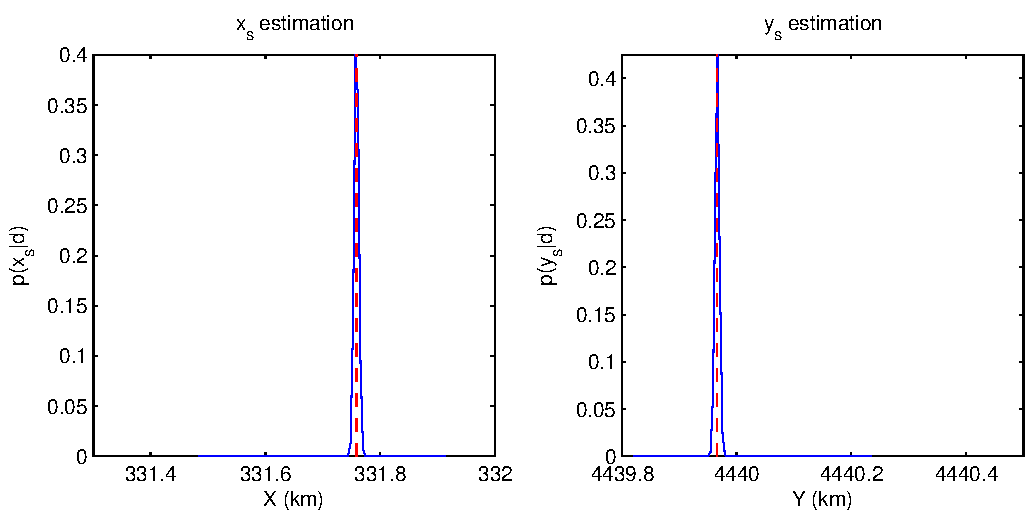
\includegraphics[width=1\textwidth]{fig_5_1}
 		\caption{Trial 7}
 		\label{fig_5_1_AE}
 	\end{subfigure}
 	\begin{subfigure}[t]{1\textwidth}
 		\centering
 		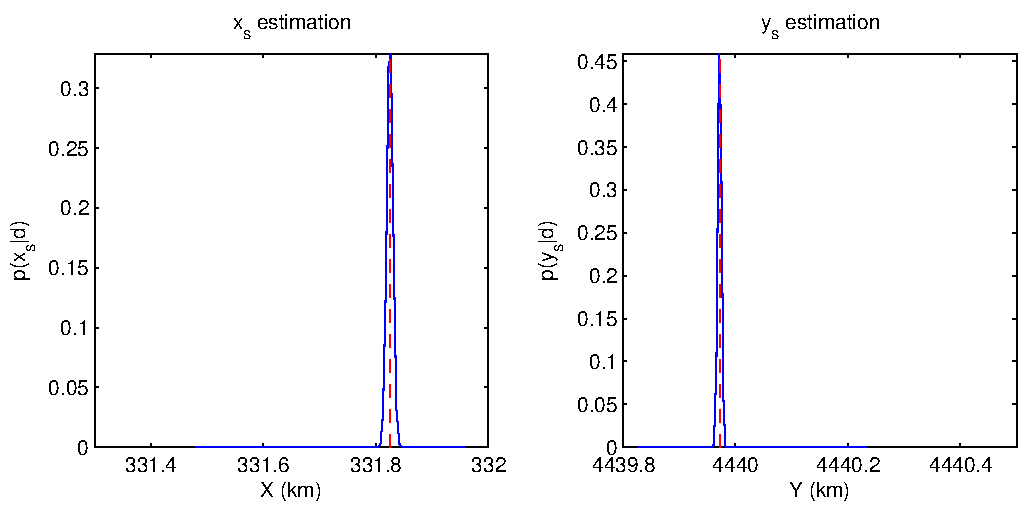
\includegraphics[width=1\textwidth]{fig_5_2}
 		\caption{Trial 30}
 		\label{fig_5_2_AE}
 	\end{subfigure}
 	\caption{Distributions a posteriori de la position de la source (en bleu) à partir de données d'observations synthétiques pour le trial 7 (\ref{fig_5_1_AE}) et le trial 30 (\ref{fig_5_2_AE}). La position réelle de la source est en pointillés rouges.}
 	\label{fig_5_AE}
 \end{figure}
 On peut voir sur la figure \ref{fig_5_AE} que l'AMIS fournit une bonne estimation de la position de la source dans chacun des \textit{trials}.\\
 
  Le fait de visualiser une distribution de probabilité permet ainsi une vision plus explicite des aspects liés aux incertitudes autour de l'estimation,  en comparaison avec des méthodes de type optimisation où seule une estimation ponctuelle est donnée.
  
  Pour obtenir les distributions présentées à la figure \ref{fig_5_AE}, {un lissage par noyau} a été effectué afin de construire une densité de probabilité à partir d'une population statistique, en l'occurence les particules $\left\{\VecTheta_k^{(i)}\right\}_{0\leq k \leq K}^{1\leq i \leq N_p}$ associées à leurs poids d'importance respectifs $\left\{\widetilde{w}_k^{(i)}\right\}_{0\leq k \leq K}^{1\leq i \leq N_p}$. \\
  
  
  Néanmoins, il est toujours possible d'obtenir un estimateur ponctuel à partir des lois a posteriori, il suffit pour cela de calculer, {par exemple}, le MMSE selon la formule suivante: 
  
  \begin{equation}
  \widehat{\PosSource} = \sum\limits_{k=0}^K\sum\limits_{i=1}^{N_p} \tilde{w}_k^{(i)}\VecTheta_{k}^{(i)}
  \end{equation}
  
  On arrive ainsi à un point estimé distant de moins d'un mètre par rapport à la position réelle de la source. \\

  \subsubsection{Estimation du profil de rejet}
  
  \NdFS{Afin de visualiser l'estimation du profil d'émission, on utilise également une approche basée sur le MMSE. L'estimation de $\VecQSource$ peut alors s'écrire:
  \begin{equation}
	  \widehat{\VecQSource} = \sum\limits_{k=1}^K \sum\limits_{i=1}^{N_p} \widetilde{w}_k^{(i)} \PostMeanQ(\VecPosSource_k^{(i)})
	  \label{eq_mmse_q}
  \end{equation}
  
  La matrice de covariance associée à cette estimation est obtenue suivant le même processus:
  \begin{equation}
	 \MatSigma_{\widehat{\VecQSource}} = \sum\limits_{k=1}^K \sum\limits_{i=1}^{N_p} \widetilde{w}_k^{(i)} \PostCovQ(\VecPosSource_k^{(i)})
  \end{equation}
}
  La figure \ref{fig_6_AE} illustre l'impact de l'utilisation de la contrainte de positivité pour l'estimation du profil du rejet $\VecQSource$.
  
 \begin{figure}[h!]
 	\centering
 	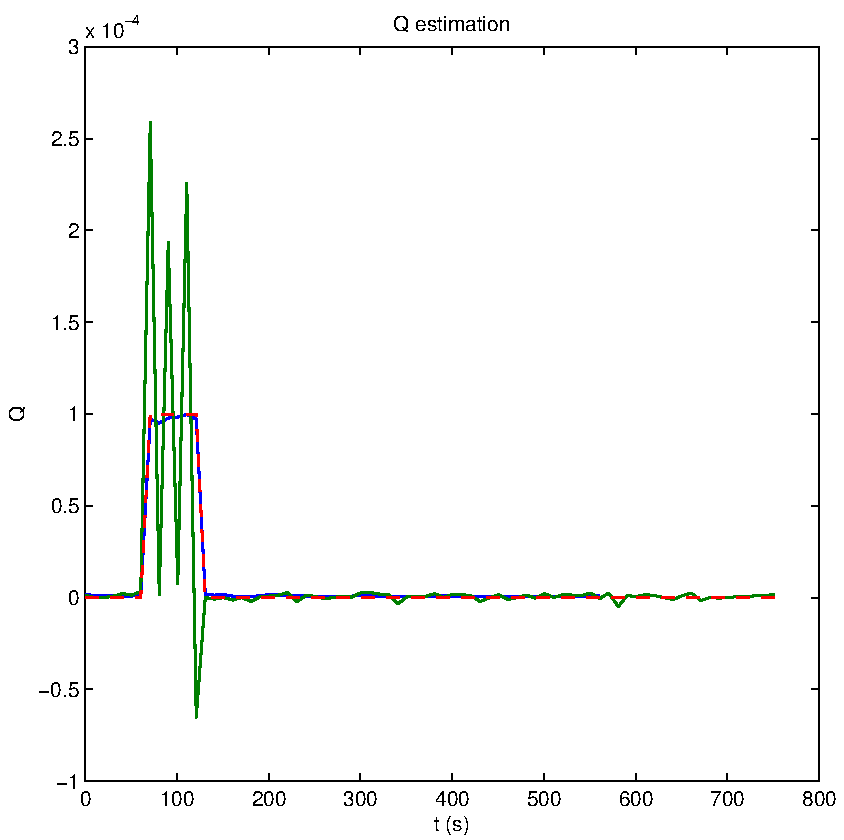
\includegraphics[width=0.5\textwidth]{fig_6}
 	\caption{Estimation de $\VecQSource$ sans (vert) et avec (bleu) application de la contrainte de positivité, comparaison avec le profil d'émission recherché (rouge).}
 	\label{fig_6_AE}
 \end{figure}
 
 L'application de la contrainte de positivité améliore le résultat de l'estimation et permet de retrouver un profil d'émission suffisamment proche de celui recherché pour avoir une bonne estimation, tant en termes d'amplitude du débit que de détection des temps d'activation et d'arrêt d'émission de la source.\\
 
 En général, du fait de sa nature potentiellement variable, le profil d'émission de la source peut prendre différents types d'allures. Nous avons ainsi modifié ce profil afin de représenter des cas non-triviaux, généré les observations correspondantes, et cherché à retrouver les caractéristiques de la source. \\
 
  \begin{figure}[h!]
  	\centering
  	\begin{subfigure}[t]{0.5\textwidth}
  		\centering
  		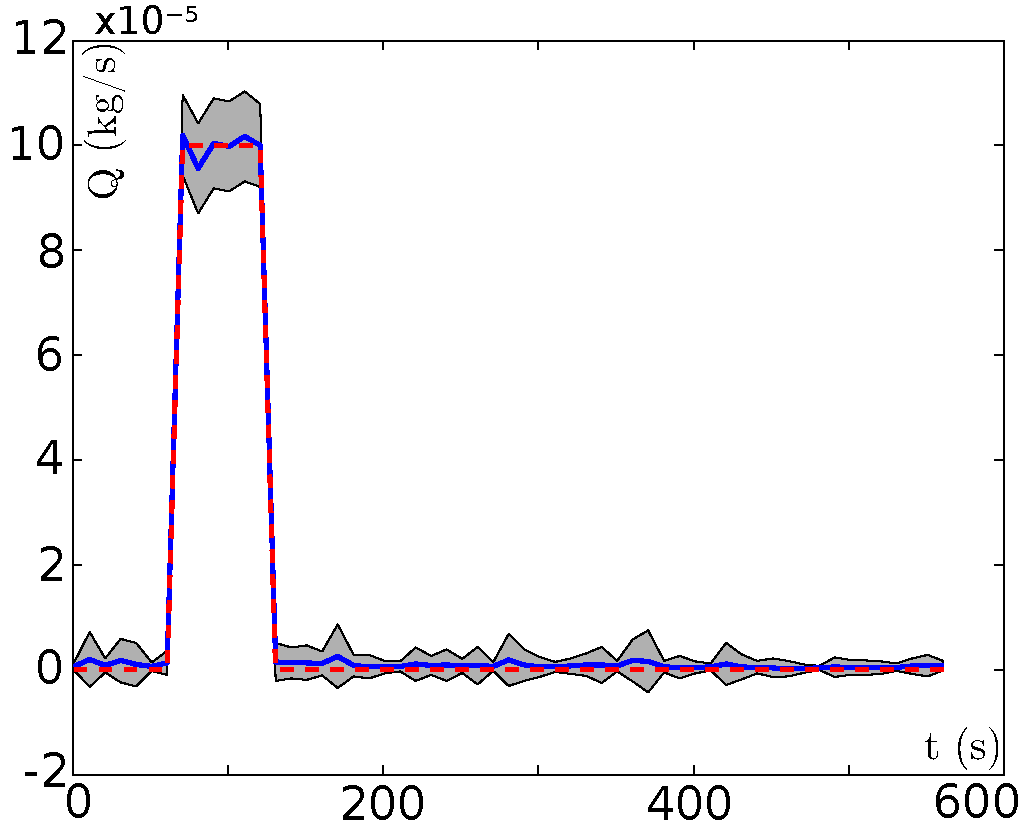
\includegraphics[width=1\textwidth]{fig_7_A}
  		\caption{}
  		\label{fig_AE_7_A}
  	\end{subfigure}%
  	\begin{subfigure}[t]{0.5\textwidth}
  		\centering
  		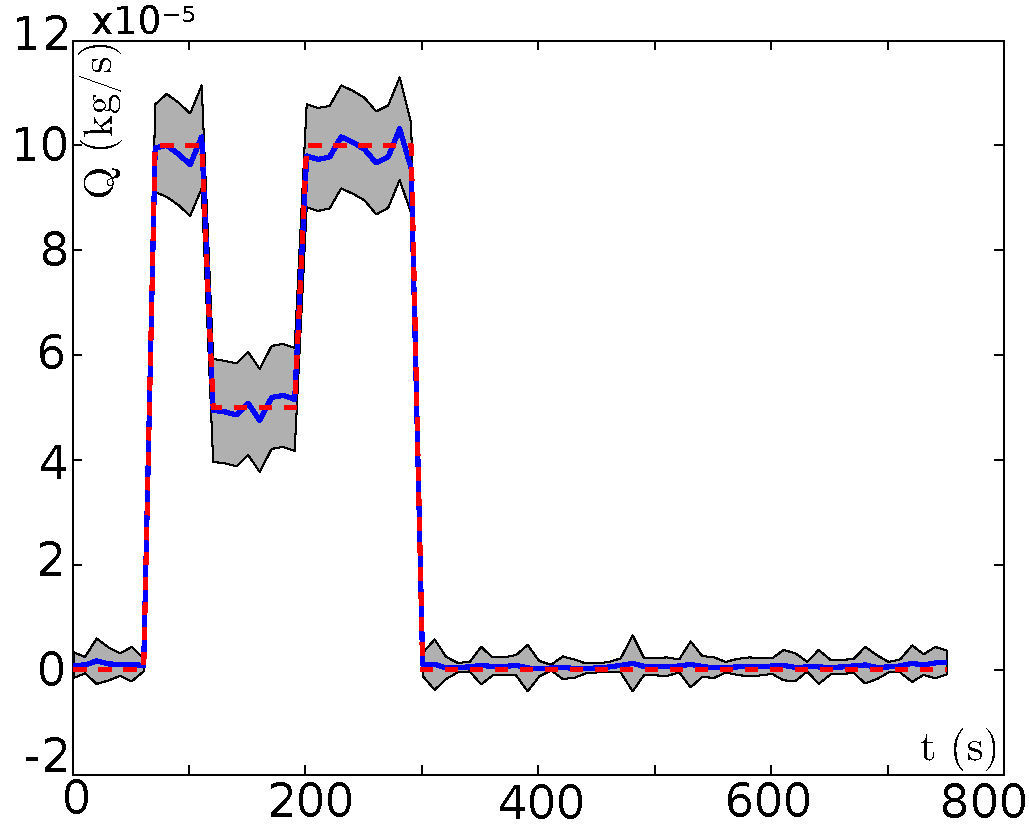
\includegraphics[width=1\textwidth]{fig_7_B}
  		\caption{}
  		\label{fig_AE_7_B}
  	\end{subfigure}
  	\begin{subfigure}[t]{0.5\textwidth}
  		\centering
  		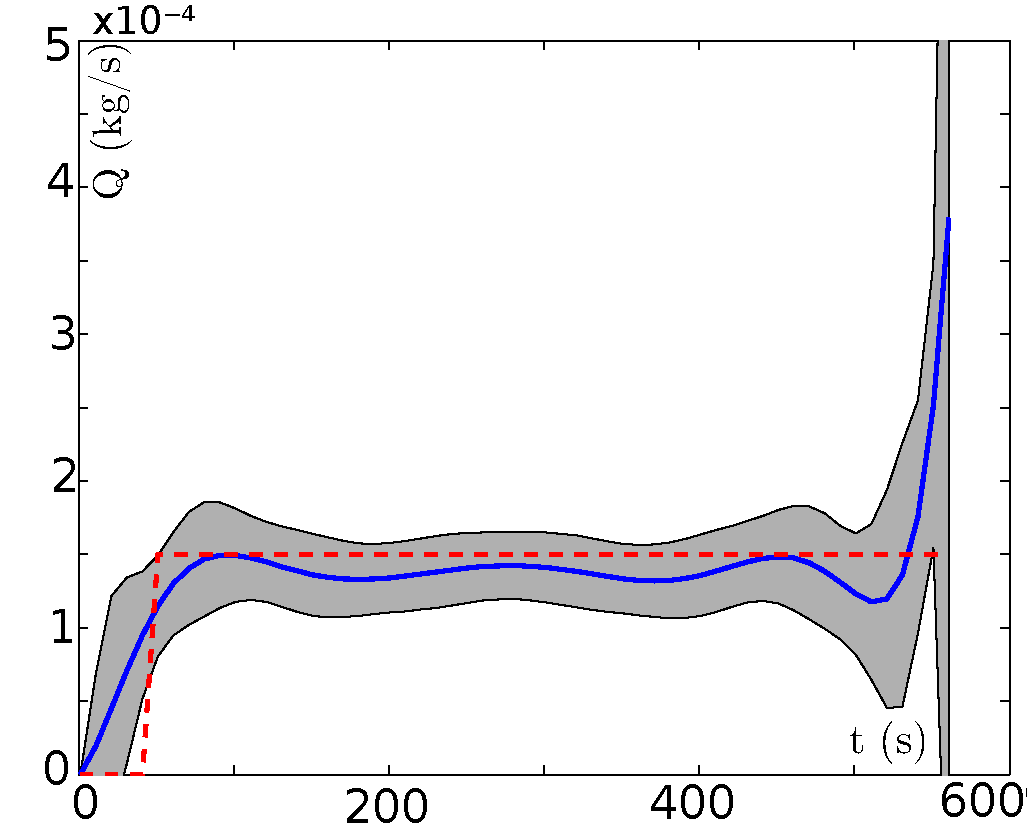
\includegraphics[width=1\textwidth]{fig_7_C}
  		\caption{}
  		\label{fig_AE_7_C}
  	\end{subfigure} 
  	
  	\caption{Simulation et résultats d'estimation pour différents profils d'émission: rejet simple (\ref{fig_AE_7_A}), rejet variable (\ref{fig_AE_7_B}), rejet continu (\ref{fig_AE_7_C}). Le profil à retrouver (en rouge) est comparé au profil estimé (en bleu) et à l'intervalle de confiance à $\pm 2 \widetilde{\sigma}_q$ (en gris).}
  	\label{fig_AE_7}	
  \end{figure}
  
  Comme présenté en figure \ref{fig_AE_7}, la méthode parvient à fournir une bonne estimation du profil de rejet dans les trois cas présentés. Sachant que l'estimation de la loi a posteriori de $\VecQSource$ \NdFS{dépend à la fois de $\PostMeanQ$ et $\PostCovQ$,} il est possible de représenter la marge d'incertitude associée à chaque valeur estimée: pour chacun des cas de la figure \ref{fig_AE_7} la valeur réelle du débit est bien incluse dans l'intervalle à $\pm 2\widetilde{\sigma}_q$, où \NdFS{$\widetilde{\sigma}_q^2 = \text{diag}(\MatSigma_{\widehat{\VecQSource}})$}. Dans le cas de la figure \ref{fig_AE_7_C}, {on observe un effet de bord sur la fin du rejet estimé, phénomène qui est absent des autres configurations. Cela est dû au fait que l'algorithme ne dispose pas des mesures permettant de confirmer ou non les valeurs non-nulles prises par le débit estimé, ces observations étant après la limite supérieure de la fenêtre temporelle d'observation. Le problème ne se pose pas dans les configurations précédentes, car comme les concentrations mesurées sont nulles au dernier instant d'observation, l'algorithme laisse la valeur de débit estimé égale à sa moyenne a priori, à savoir 0.}
  
  
  le pic à la limite de l'intervalle d'émission est dû au fait que le rejet est plus long que la période d'observation: en l'absence d'information, l'algorithme ne peut fournir une estimation correcte, mais demeure cohérent  en augmentant fortement la taille de la marge d'incertitude, signifiant ainsi que l'information manque. \\
  
  \subsubsection{Robustesse statistique de l'estimation}
    
    L'algorithme AMIS est une procédure basée sur l'échantillonnage d'importance, qui est par nature une démarche aléatoire. Pour tenir compte de cette caractéristique dans la validation de notre méthodologie, nous avons exécuté l'AMIS sur plusieurs \textit{runs}, avec et sans application de la contrainte de positivité, et en perturbant les observations de concentrations fournies. Nous avons ensuite comparé les performances dans chacun des cas, en analysant les résultats présentés au tableau \ref{table_1_AE}. 
    
    \begin{table}[h!]
    	\centering
    	
    	\begin{tabular}{cccc}
    		
    		Contrainte de positivité & $\bar{d}(\widehat{\PosSource},\PosSource)$ (m)& $\sigma_{\widehat{x_s}}$ (m)& $\sigma_{\widehat{y_s}}$ (m)\\
    		\hline
    		OUI                   & {$<1$}  	& 0.9        & 3.2        \\
    		NON                   & 10.44   & 0.4        & 1.0 \\      
    		\hline
    	\end{tabular}
    	\caption{Evaluation statistique des estimations sur 40 runs de l'AMIS avec et sans application de la contrainte de positivité. $\bar{d}(\widehat{\PosSource},\PosSource)$ représente la distance moyenne entre la position de source estimée par MMSE et l'emplacement réel de la source. $\sigma_{\widehat{x_s}}$ et $\sigma_{\widehat{y_s}}$ sont respectivement les moyennes des écarts-types des distributions a posteriori marginales $p(x_s | \VecObs)$ et $p(y_s | \VecObs)$. }
    	\label{table_1_AE}
    \end{table}
    
    Ces résultats confirment que l'application de la contrainte de positivité apporte en moyenne une certaine amélioration au niveau de la localisation de la source. Si on cherche à quantifier la précision de l'estimation du profil de rejet, on peut calculer l'erreur quadratique moyenne, ou \textit{mean square error} (MSE), entre la valeur estimée \NdFS{$\widehat{\VecQSource}$} et la valeur théorique $\VecQSource$ selon la formule suivante: 
    \NdFS{
    \begin{equation}
    \text{MSE}(\widehat{\VecQSource}, \VecQSource) = \dfrac{1}{T_s}\sum\limits_{n=1}^{T_s}\left(\widehat{\VecQSource}(t'_n) - \VecQSource(t'_n)\right)^2
    \label{eq_AE_31}
    \end{equation}
}
Dans le cas où on applique la contrainte de positivité, on a une erreur MSE de $1.37\times10^{-12}$, qui est une meilleure valeur que pour le cas sans contrainte, où on a une erreur MSE de $1.26\times10^{-9}$.  \\

\subsubsection{Comparaison avec le MCMC}

Nous avons ensuite cherché à comparer les performances de l'AMIS avec un autre algorithme d'inférence bayésienne couramment utilisé pour les problèmes STE, en l'occurence la méthode MCMC, présentée dans le Chapitre 2. \\

Pour cela, nous avons implémenté une algorithme de type \textit{random walk Metropolis}  avec un noyau de transition gaussien fixe, et l'intégration de la contrainte de positivité de l'algorithme \ref{algo_PCO} dans le calcul de la vraisemblance, sur 1000 itérations. Afin de tenir compte du phénomène de \textit{burn-in}, les 100 premiers états sont ignorés. \\

Un test de robustesse statistique a ensuite été effectué, en changeant de façon aléatoire le point de départ de la chaîne de Markov à chaque \textit{run} (uniformément sur le domaine). Pour la localisation de la source, l'estimateur MMSE moyen obtenu par MCMC a été comparé aux résultats de l'AMIS dans le tableau \ref{table_2_AE}. \\

    \begin{table}[h!]
    	\centering
    	
    	\begin{tabular}{cccc}
    		
    		Algorithme &{ $\bar{d}(\widehat{\PosSource},\PosSource)$ (m)}& $\sigma_{\widehat{x_s}}$ (m)& $\sigma_{\widehat{y_s}}$ (m)\\
    		\hline
    		AMIS                   & {$<1$}  	& 0.9        & 3.2        \\
    		MCMC                   & {22.7}  & 130        & 95 \\      
    		\hline
    	\end{tabular}
    	\caption{Evaluation statistique des estimations sur 40 \textit{runs} de l'AMIS et du MCMC avec application de la contrainte de positivité.}
    	\label{table_2_AE}
    \end{table}
    
 Dans cette étude de cas, on remarque ainsi que les performances de l'AMIS sont meilleures en termes de précision pour localiser la source. De fait, l'approche MCMC est en partie pénalisée par l'étape d'initialisation. En effet, la convergence vers une position suffisamment proche de la vraie source est d'autant plus longue et incertaine que l'état initial de cette chaîne est éloigné de la vraie source. En ce sens, le fait de travailler sur une population de particules plutôt que sur la succession d'états séquentiels, ainsi que l'aspect adaptatif de l'AMIS lui permettent une meilleure flexibilité pour la mise à jour des paramètres de la loi de proposition, réduisant ainsi la dépendance de ses performances par rapport à l'état initial. Une alternative serait d'instancier plusieurs chaînes de Markov dont les états initiaux sont suffisamment éloignés les uns des autres pour bien couvrir le domaine, mais cela augmente la charge de calcul et les ressources requises pour l'exécution de l'algorithme. \\
 
 En plus de la précision de chacun des algorithmes, nous nous sommes également penchés sur leur vitesse de convergence. \\
 
 \begin{figure}[h!]
 	\centering
 	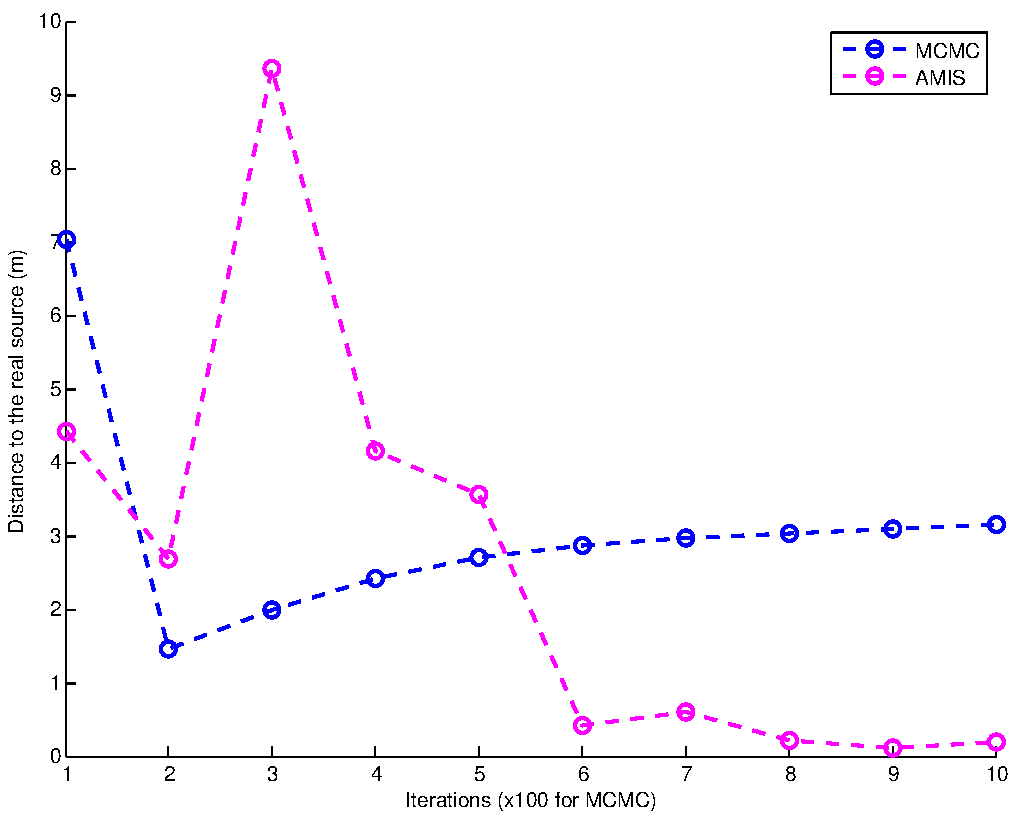
\includegraphics[width=0.7\textwidth]{fig_8}
 	\caption{Comparaison empirique de la vitesse de convergence entre MCMC (en bleu) et AMIS (en magenta)}
 	\label{fig_8_AE} 	
 \end{figure}

 Sur la figure \ref{fig_8_AE}, on utilise un critère qualitatif qui est la distance de l'estimation MMSE du lieu du rejet à une itération donnée. Les calculs ont été calibrés afin que chacun des algorithmes traite une charge équivalente de calcul. Ainsi, avec:
 \begin{itemize}
 	\item $N_p=100$ particules par itérations et $K=10$ itérations pour l'AMIS,
 	\item $1000$ itérations pour le MCMC,
 \end{itemize} 
 le nombre de calculs de la loi de vraisemblance, et par extension le nombre d'appels au modèle de dispersion, est strictement le même pour les deux algorithmes. \\
 
 Les résultats obtenus démontrent l'efficacité de l'aspect adaptatif de l'AMIS, qui lui permet d'atteindre rapidement une estimation de bonne qualité pour la localisation de la source.\\
 
 Encore une fois, dans la démarche MCMC, l'initialisation de la chaîne de Markov influe sur la vitesse de convergence, cette dernière étant d'autant plus élevée que l'état initial se situe près de la vraie source. Un autre paramètre du MCMC intervient également ici: la variance du noyau de transition. En effet, comme expliqué au Chapitre 2, si la valeur choisie pour cette variance est trop faible, même si l'initialisation place la chaîne dans une position relativement favorable, la convergence sera trop lente car le nombre d'états nécessaires pour atteindre une estimation correcte sera plus élevé. A l'inverse, il est risqué de trop augmenter la valeur de cette variance, car cela entraînerait des transitions d'amplitude trop élevée, pouvant potentiellement empêcher la convergence vers le point source recherché. L'AMIS est quant à lui plus souple dans sa démarche de transition d'une itération à l'autre, cependant il peut être également sujet à des problèmes de convergence si, par exemple, les particules échantillonnées par la loi de proposition initiale ne couvrent pas du tout la zone où se situe la vraie source, d'où l'intérêt d'une initialisation homogène telle que présentée à la figure \ref{init_amis_good}.\\
 
 \subsubsection{Effective Sample Size}
 
 Un critère spécifique aux méthodes basées sur l'échantillonnage d'importance est la représentativité de la distribution cible en fonction des particules ayant été échantillonnées afin d'approximer cette loi. Un outil permettant de quantifier cette grandeur est l'ESS, tel que présenté à l'équation \eqref{eq_def_ESS}, il permet ici en particulier de surveiller si l'AMIS est bloqué par un effet de dégénérescence des poids, ce qui se manifeste par une valeur d'ESS constamment faible. \\
 
 \begin{figure}[h!]
 	\centering
 	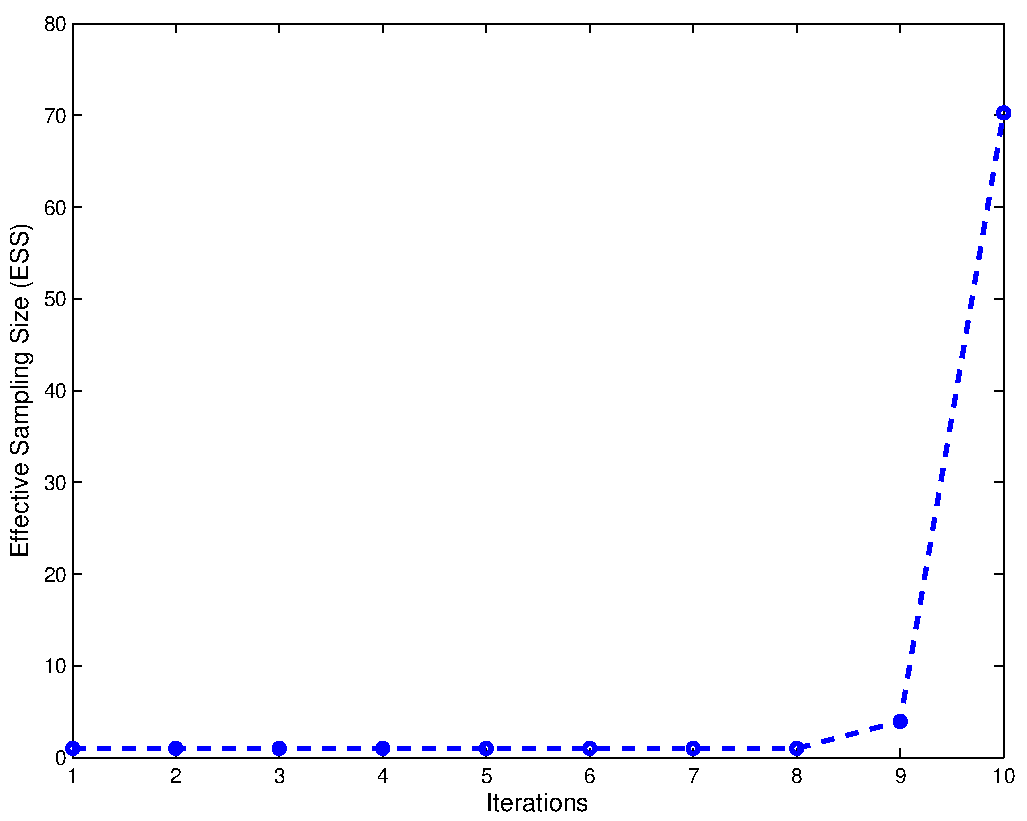
\includegraphics[width=0.7\textwidth]{fig_9}
 	\caption{Evolution de l'ESS par itération (avec $N_p=100$ particules tirées par itération)}
 	\label{fig_9_AE}
 \end{figure}
 
 On observe sur la figure \ref{fig_9_AE} que l'ESS prend un certain {nombre d'itérations} avant d'atteindre des valeurs suffisamment élevées, néanmoins l'estimation de la position de la source devient rapidement pertinente si on se réfère à la figure \ref{fig_8_AE}. En pratique, cela illustre le fait que l'AMIS a tendance à affecter un poids relativement élevé à un nombre restreint de particules (voire à une particule unique) proches de la vraie source. 
 
 
 \subsection{Résultats obtenus avec des données expérimentales}
 
 Après un premier ensemble de tests sur données simulées, nous avons appliqué la même méthodologie en utilisant les mesures de concentrations expérimentales directement issues de l'expérience FFT07. \\
 
 \subsubsection{Traitement des données manquantes}
 
 Une première analyse des données d'observation a permis de mettre en évidence l'absence de mesures de concentrations sur certaines plages temporelles, voire sur la totalité de la fenêtre d'observation, pour plusieurs capteurs du réseau, dans les \textit{trials} 7 et 30. Ces données manquantes sont le résultat de défaillances ponctuelles des dispositifs instrumentaux au moment des essais. Nous avons ainsi eu à gérer deux types de situations:
 
 \begin{itemize}
 	\item Dans les cas où les données sont partiellement manquantes, typiquement s'il existe une quantité finie de points de mesure où les concentrations ne sont pas disponibles, alors une interpolation linéaire est faite pour remplir les valeurs manquantes à partir des concentrations disponibles.
 	\item Dans les cas où aucune concentration n'est disponible sur un capteur donné, ce dernier est écarté du réseau et n'est pas intégré au vecteur d'observations $\VecObs$. La même opération est faite si la proportion des points de mesures manquants est significativement supérieure à la quantité de mesures valables, l'opération d'interpolation étant dans ces cas-à susceptible d'introduire une information faussée.\\
 \end{itemize}
 
\subsubsection{Variabilité météorologique}

Le fait d'utiliser des données expérimentales permet également de prendre en compte la présence de variations de vitesse et de direction du vent, et voir si l'algorithme d'estimation de la source arrive à gérer une telle situation. En particulier dans le \textit{trial} 7, la direction du vent change sensiblement durant la période du rejet, comme le montre la figure \ref{fig_11_AE}.

\begin{figure}[h!]
	\centering
	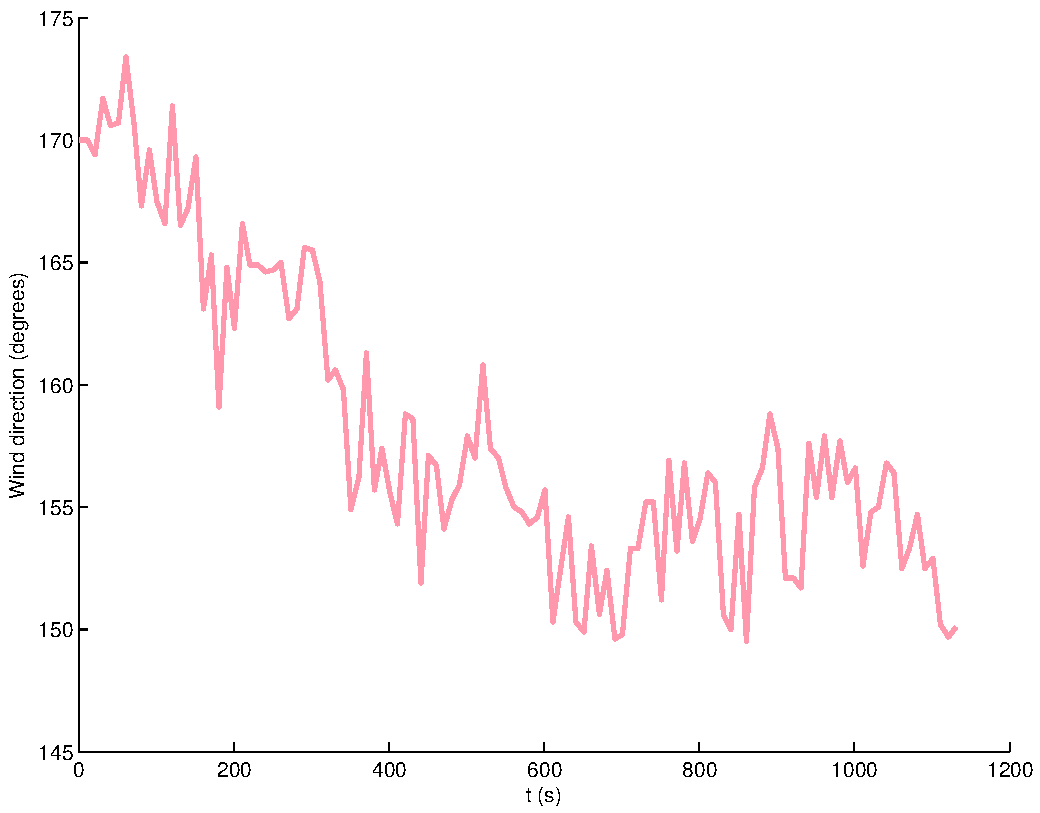
\includegraphics[width=0.7\textwidth]{fig_11}
	\caption{Direction du vent mesurée par la station météorologique la plus proche de la source (\textit{trial} 7)}
	\label{fig_11_AE}
\end{figure}

Le choix d'un modèle de dispersion à bouffées gaussiennes permet ainsi d'intégrer ces variations de vent: pour le \textit{trial} 7 nous avons donc recueilli et moyenné les mesures de vent issues des deux capteurs de vent soniques (anémomètres à ultrasons) présents sur le domaine, puis intégré les valeurs résultantes dans le modèle de dispersion. Pour le \textit{trial} 30 les variations sont beaucoup moins importantes, nous avons donc gardé l'hypothèse d'un vent stationnaire uniforme. \\

\subsubsection{Estimation de la position (\textit{trials} 7 et 30)}

De même que pour le cas synthétique, nous avons {obtenu} par KDE les distributions a posteriori de la position de la source sur chacun des axes, et représenté les résultats pour les \textit{trials} 7 et 30 sur les figures \ref{fig_12_AE} et \ref{fig_13_AE}. Les paramètres suivants ont été utilisés:

\begin{itemize}
	\item \textit{trial} 7: $\varObs = 10^{-10}$ et $\varQ = 5\times 10^{-2}$,
	\item \textit{trial} 30: $\varObs = 5 \times 10^{-8}$ et $\varQ = 5\times 10^{-3}$.\\
\end{itemize}

\begin{figure}[h!]
	\centering
	\begin{subfigure}[t]{0.5\textwidth}
		\centering
		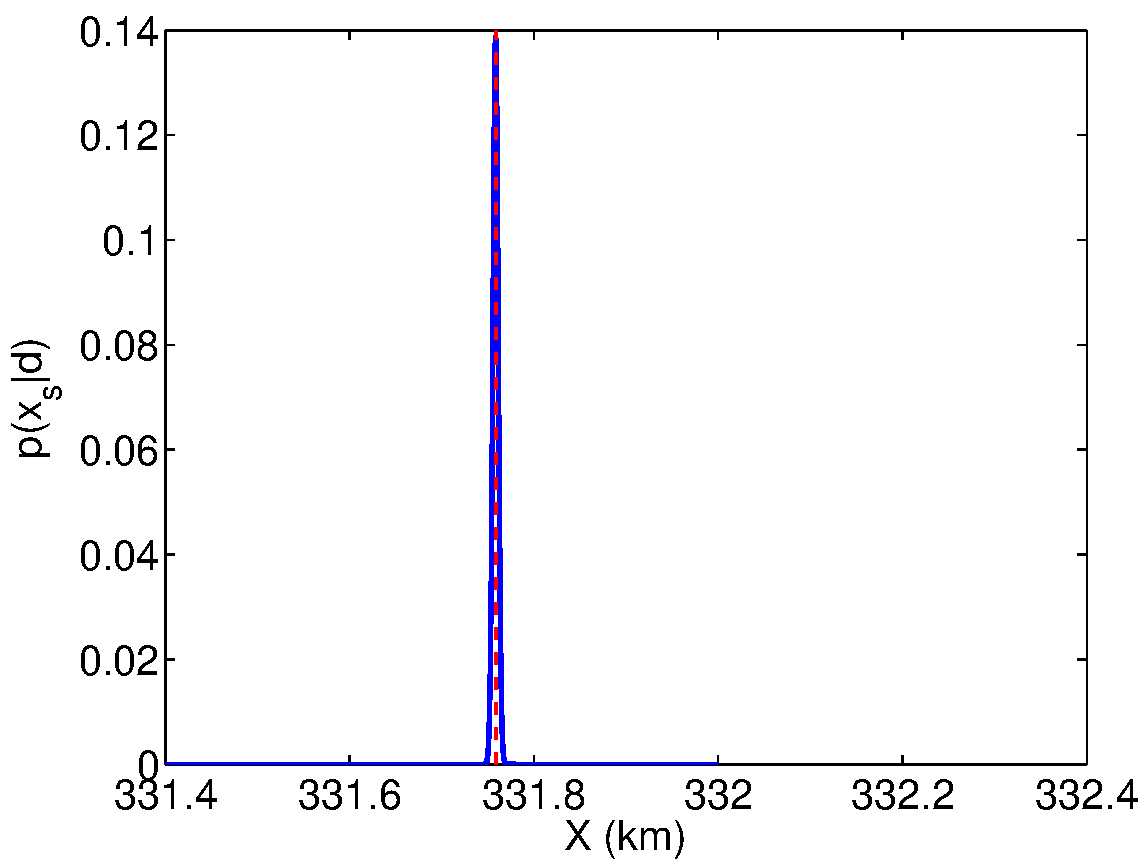
\includegraphics[width=1\textwidth]{fig_12_A}
		\caption{}
		\label{fig_12_A}
	\end{subfigure}%
	\begin{subfigure}[t]{0.5\textwidth}
		\centering
		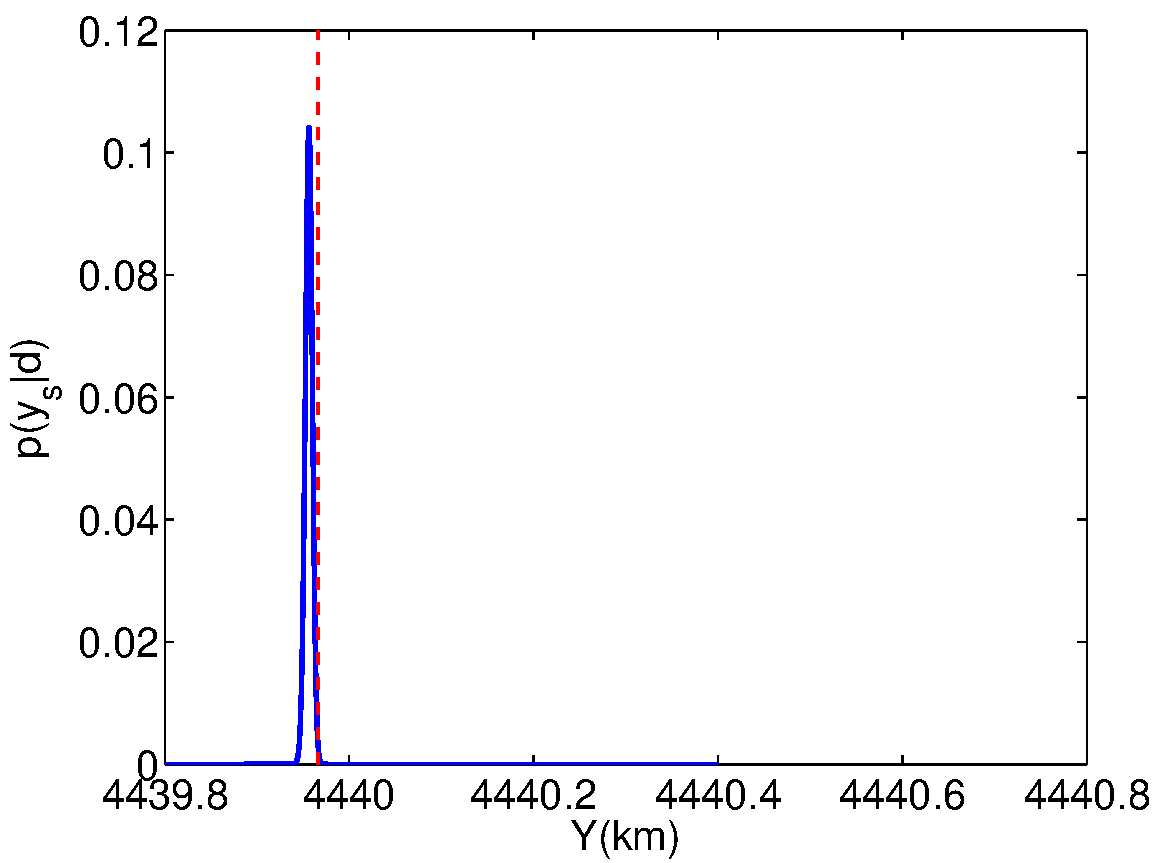
\includegraphics[width=1\textwidth]{fig_12_B}
		\caption{}
		\label{fig_12_B}
	\end{subfigure}
	\caption{Distribution a posteriori de la position de la source (en bleu) à partir des données d'observations expérimentales FFT07 pour le \textit{trial} 7. La position réelle de la source est en pointillés rouges.} 
	\label{fig_12_AE}		
\end{figure}

\begin{figure}[h!]
	\centering
	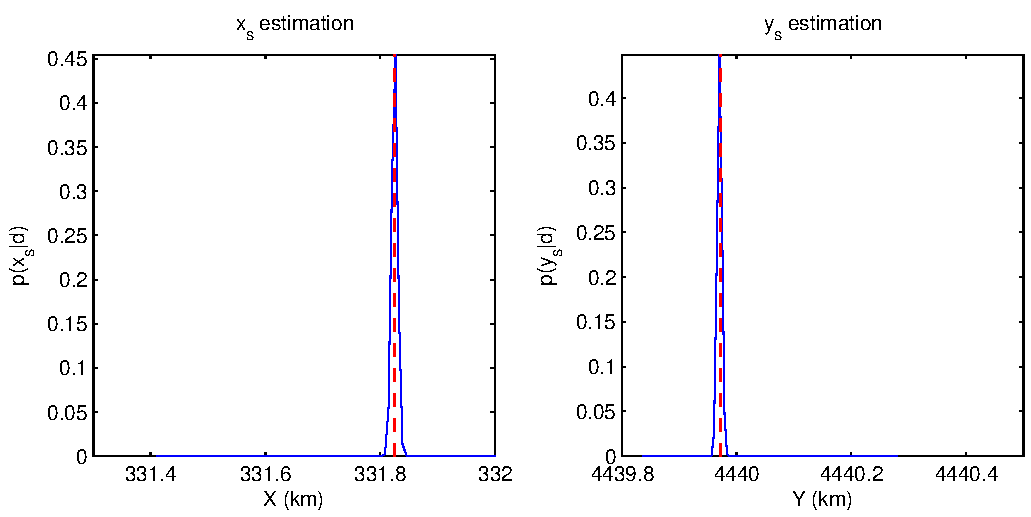
\includegraphics[width=1\textwidth]{fig_13}
	\caption{Distribution a posteriori de la position de la source (en bleu) à partir des données d'observations expérimentales FFT07 pour le \textit{trial} 30. La position réelle de la source est en pointillés rouges.}
	\label{fig_13_AE}
\end{figure}

On observe que les résultats sont presque aussi bons que dans le cas synthétique. En termes de distance de l'estimée ponctuelle MMSE par rapport à la vraie source, on reste sur des valeurs satisfaisantes de 9.8m pour le \textit{trial} 7 et 1.5m pour le \textit{trial} 30. 

\subsubsection{Comparaison avec le MCMC (\textit{trial} 7)}

Une comparaison avec le même type d'algorithme MCMC que le paragraphe §\ref{par_simule} a également été menée, en utilisant les données expérimentales du \textit{trial} 7. On remarque sur la figure \ref{fig_14_AE} que pour l'estimation de la position, les deux méthodes fournissent des résultats globalement satisfaisants. \\

\begin{figure}[h!]
	\centering
	\begin{subfigure}[t]{0.5\textwidth}
		\centering
		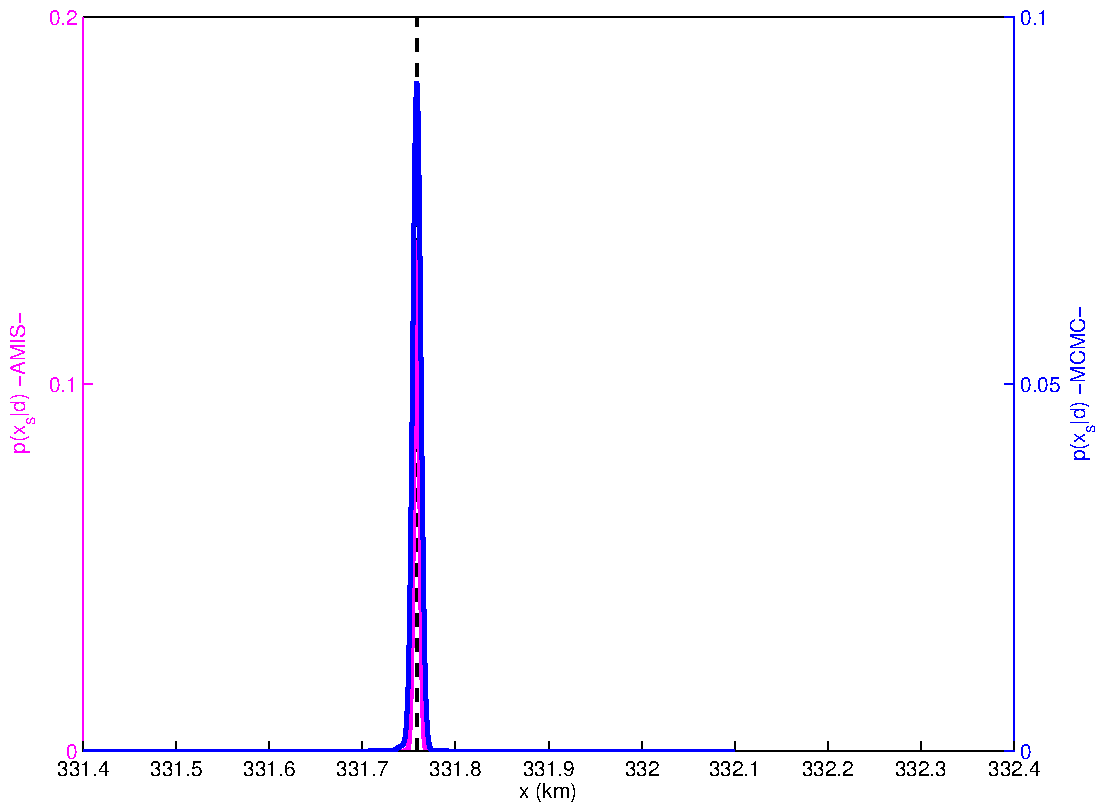
\includegraphics[width=1\textwidth]{fig_14_A}
		\caption{}
		\label{fig_14_A}
	\end{subfigure}%
	\centering
	\begin{subfigure}[t]{0.5\textwidth}
		\centering
		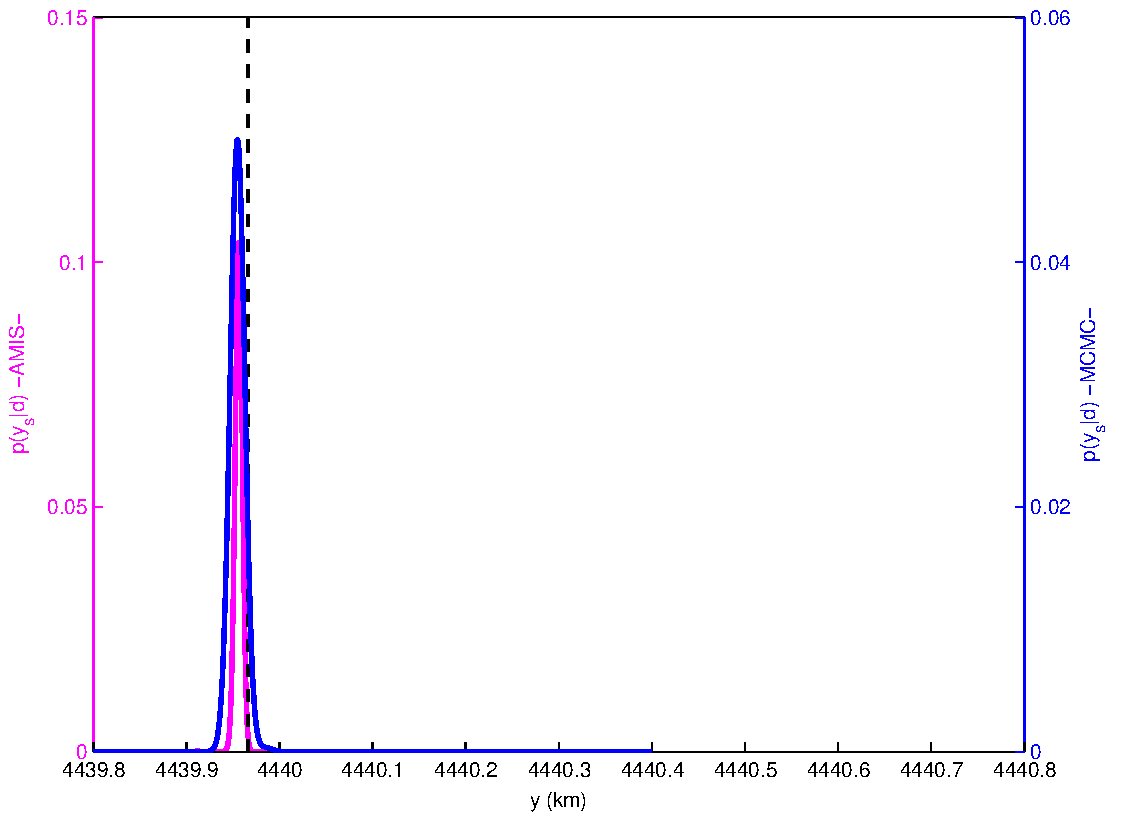
\includegraphics[width=1\textwidth]{fig_14_B}
		\caption{}
		\label{fig_14_B}
	\end{subfigure}
	\caption{Comparaison de l'estimation de la position de la source du \textit{trial} 7 avec des observations réelles en utilisant AMIS (en magenta) et MCMC (en bleu). La position réelle de la source est en pointillés noirs.}
	\label{fig_14_AE} 
\end{figure}

La comparaison a aussi été faite avec les résultats d'estimation du profil de rejet, comme illustré en figure \ref{fig_15_AE}. Les résultats ont été moyennés sur des fenêtres d'1 minute afin de lisser l'allure du débit.

 On note que les premières valeurs non-nulles du débit estimé apparaissent plus tôt qu'attendu, et avec des amplitudes plus importantes. Cela est en partie causé par le fait que l'estimée ponctuelle de la source a été située  en amont de la position réelle, ce qui a forcé l'algorithme à produire un débit plus important pour ajuster en conséquence les concentrations résultantes au niveau des capteurs, et à avancer l'instant de "démarrage" du rejet. Ce phénomène est un peu plus marqué dans le cas du MCMC (\ref{fig_15_B}).

\begin{figure}[h!]
	\centering
	\begin{subfigure}[t]{0.5\textwidth}
		\centering
		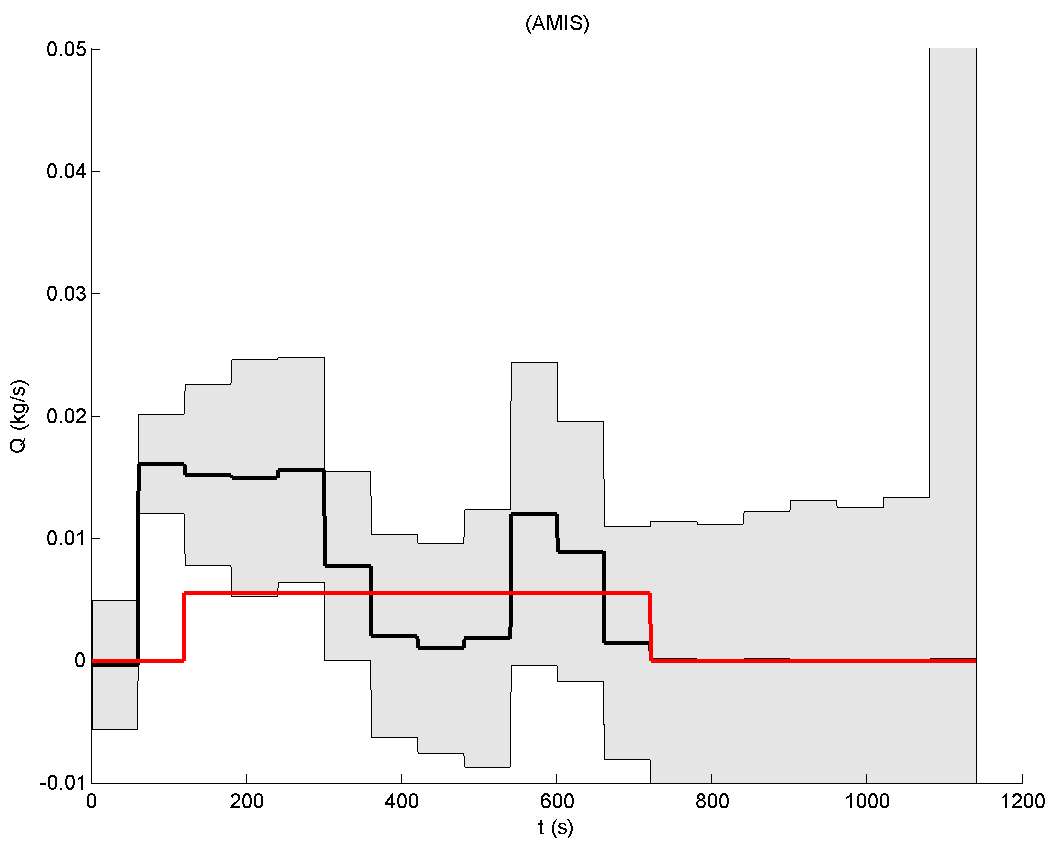
\includegraphics[width=1\textwidth]{fig_15_A}
		\caption{AMIS}
		\label{fig_15_A}
	\end{subfigure}%
	\centering
	\begin{subfigure}[t]{0.5\textwidth}
		\centering
		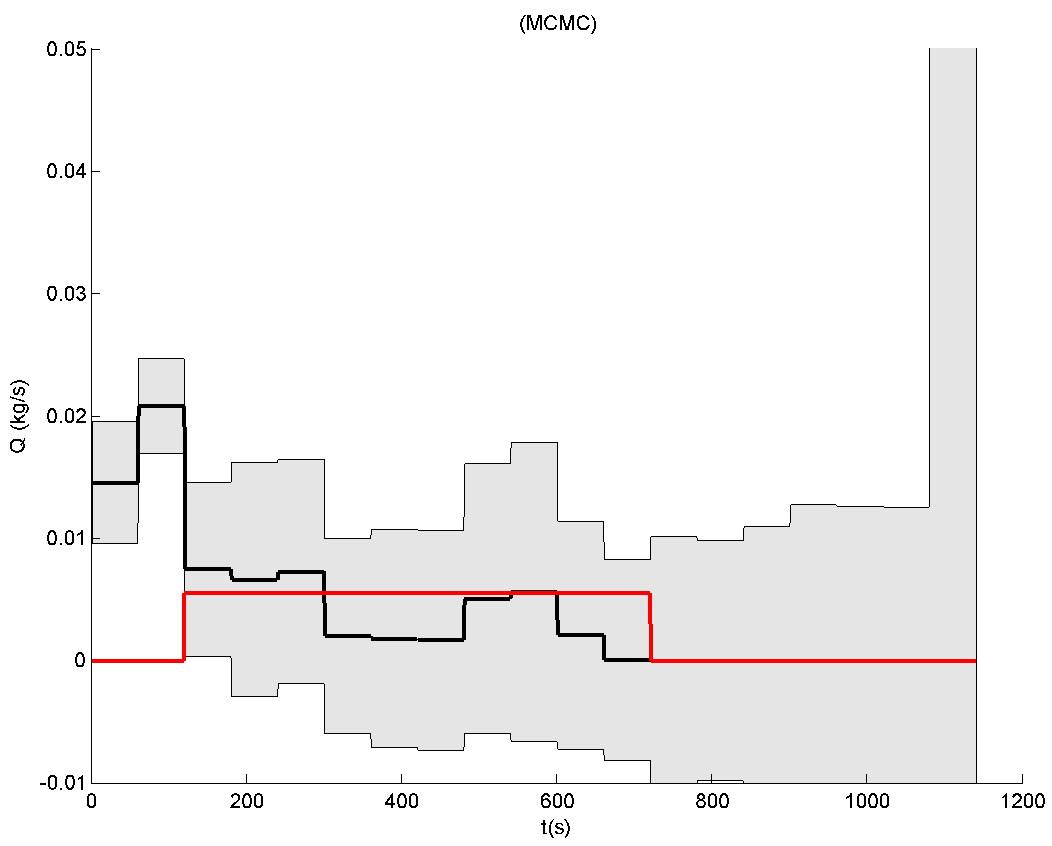
\includegraphics[width=1\textwidth]{fig_15_B}
		\caption{MCMC}
		\label{fig_15_B}
	\end{subfigure}
	\caption{Estimation du profil d'émission du \textit{trial} 7 (en noir), intervalle de confiance à $\pm 2\widetilde{\sigma}_q$ (en gris) et comparaison avec les valeurs réelles (en rouge), avec AMIS (\ref{fig_15_A}) et MCMC (\ref{fig_15_B}).}
	\label{fig_15_AE} 
\end{figure}

\section{Conclusions}

L'étude de cas sur l'expérience FFT07 présentée dans ce chapitre a permis une première validation de la méthodologie axée sur l'algorithme AMIS. Celle-ci a en effet permis une bonne estimation de la position de la source dans les cas synthétiques et expérimentaux,  en fournissant une distribution a posteriori des coordonnées de la source. Cet outil statistique permet ainsi d'effectuer une analyse autour des incertitudes associées à l'estimation, {tout en permettant un accès à l'information ponctuelle} par le biais du calcul de l'estimateur MMSE. \\

 La démarche et a également permis de reconstruire un profil d'émission complet, fournissant une information temporelle sur les quantités émises par la source ainsi que ses temps de démarrage et d'arrêt. Cet aspect temporel présente un aspect innovant par rapport aux approches conventionnelles présentées dans la littérature, où l'hypothèse d'un débit d'émission constant est formulée, se traduisant dans la pratique par la recherche d'une unique valeur scalaire $q$. 
 
Cette étude a démontré que la quasi-totalité de la charge de calcul est concentrée sur la construction des matrices source-récepteur, plus précisément sur les appels au modèle de dispersion. Dans le cas d'un modèle gaussien les temps de calcul demeurent raisonnables, mais ils dépendent directement du nombre de particules échantillonnées par itération de l'AMIS. Nous avons pu vérifier que le fait de tirer plus de 100 particules par itération dans cette étude de cas n'améliorait pas significativement les résultats d'estimation {en termes de précision}, mais dans le cadre général un nombre trop faible de particules pourrait dégrader la qualité de l'estimation, car l'exploration de l'espace des paramètres s'en trouverait restreinte. De plus, à nombre égal de particules, si le contexte exige l'utilisation d'un modèle de dispersion plus élaboré (par exemple dans un milieu urbain), la charge et le temps de calcul seront bien plus importants. \\

{Il devient ainsi nécessaire d'optimiser à la fois le mode d'usage du modèle de dispersion ainsi que l'exploration des différentes valeurs possibles pour les particules. Ces deux points sont abordés dans le Chapitre 4, qui présente une nouvelle façon d'obtenir les résultats des calculs de dispersion, ainsi qu'une initialisation améliorée de la loi de proposition.}


